\documentclass[12pt]{article}
\usepackage[left=1.15in, right=1.15in, top=1in, bottom=1.5in]{geometry}
\usepackage{natbib}
\usepackage{verbatim}
\usepackage{setspace}
\usepackage{booktabs}
\usepackage{caption}
\usepackage{graphicx}
\usepackage{subcaption}
\bibpunct[: ]{(}{)}{;}{a}{}{,} 
\usepackage{authblk}
\renewcommand\Authfont{\normalsize}
\renewcommand\Affilfont{\footnotesize}

\begin{document}
\title{The Forward March of Categorical Tolerance in the United States\thanks{Reserved for acknowledgments}}
\author[1]{Omar Lizardo\thanks{olizardo@soc.ucla.edu}}
\affil[1]{Department of Sociology, UCLA}

\renewcommand\Authands{ and }

\date{\normalsize \today}	
\maketitle

\newpage
\begin{abstract}
\end{abstract}
\newpage
\section*{Introduction}
Ever since Richard Peterson introduced the felicitous term ``patterns of cultural choice'' into sociological discourse more than four decades ago \citep{peterson1983patterns-f85}, sociologists have been busy empirically uncovering and debating the sociological reality, drivers, and correlates of various such patterns. These include, most famously and influentially, the Petersonian cultural \textit{omnivore} \citep{peterson1996changing-967, goldberg2011mapping-77a, warde2008omnivorous-e77} along with their evil twin the culturally exclusive \textit{univore} \citep{bryson1997what-933, peterson1992understanding-ce3, tonkovi2025globallocal-96f}, but also culturally \textit{voracious} consumers \citep{sullivan2007omnivore-018}, \textit{poly-purists} and \textit{poly-mixers} \citep{goldberg2016what-4e3, poecke2018pure-873}, \textit{decisives} and \textit{indecisives} \citep{sonnett2004musical-961}, and even plain old \textit{snobs} engaging in (presumably) Bourdieusian boundary-drawing distinction \citep{atkinson2011context-d44, nault2021social-1bf}, among many others.

In a paper published almost a decade ago, \citet{lizardo2016end-4fb}---hereafter L\&S---introduced another such pattern of cultural choice, which they labeled \textit{categorical tolerance}, to refer to the phenomenon of a growing proportion of the population who refuse to report dislikes of \textit{any} cultural genres---typically musical genres---in standard social science surveys designed to measure patterns of cultural taste. In that paper, L\&S noted that categorical tolerance appeared to be on the rise in the United States, going from about five percent of the population in the canonical 1993 General Social Survey culture module dataset to about sixteen percent in a then-recent survey of a representative sample of Americans collected in 2012, which matched the GSS 1993 battery of items on likes and dislikes of musical tastes across eighten genres. This resulted in a significant shift in the shape of the univariate count distributions of number of dislikes, which went from a standard Poisson distribution in the GSS 1993 to a count distribution with excess zeroes in 2012 \citep[p.90, Figure 1]{lizardo2016end-4fb}. 

In the same paper, L\&S also showed that the rise of categorical tolerance among Americans was a socially patterned phenomenon. Particularly, L\&S showed that refusal to dislike was a growing trend among more recently born cohorts, suggestive of a macro-level pattern of cultural change via cohort replacement of the type that has been more recently shown to govern macro-level cultural change across a wide variety of values, attitudes, beliefs, and practices \citep{vaisey2016cultural-867, kiley2020measuring-123, ochoa2024opinions-856, vaisey2021model-based-deb}. Moreover, when comparing 2012 to 1993 data, L\&S found that categorical tolerants were over-represented among non-white respondents, with a slight under-representation of people with a college degree, indicating that categorical tolerance did not seem to be driven by the usual status and cultural-capital-based dynamics emphasized by Bourdieusian models of social distinction \citep{bourdieu1984distinction-835}, which usually focuses on status display among higher educated elites \citep{jarness2017im-001, khan2011privilege-68a}.

This paper uses recently collected data from a representative sample of the American population to update the empirical picture of categorical tolerance in the United States for the third decade of the twenty-first century. First, I ask whether we can observe a continued rise in the categorical tolerance effect in the more recent data. Secondly, I examine the socio-demographic correlates of categorical tolerance to determine whether this pattern of cultural choice persists in a similar socio-demographic ``niche'' \citep{mcpherson2004blau-9fe} as L\&S observed in 2012, or whether its location in social space has evolved since then. Third, I also examine the socio-demographic correlates of \textit{symbolic exclusion} among people at risk of expressing dislikes \citep{bryson1996anything-311}, to see if we can observe similar patterns to those previously uncovered by L\&S. Finally, the paper adds a missing dimension to previous work on categorical tolerance and symbolic exclusion by investigating whether these cultural taste patterns are connected to political identification as liberal or conservative, given recent work indicating that cultural taste patterns have themselves become embroiled in the ``oil spill'' produced by the continuing political polarization of the American mass publics in the last two decades. This phenomenon has accelerated in the Trump era \citep{dellaposta2020pluralistic-ed4, rawlings2023polarization-0af}.

To preview the main results: I find that categorical tolerance has indeed continued its onward march among Americans, with about twenty percent of respondents failing to report disliking any of the twelve genres in data collected from two survey samples in two separate platforms. Secondly, the social location of categorical tolerance is fairly similar to that observed by L\&S a decade ago; younger adults are overrepresented among categorical tolerants relative to older adults. Similarly, as L\&S found in 2012, non-white respondents are overrepresented among categorical tolerants in the United States. One distinct difference between the current findings and L\&S's results, however, is a seeming trickle-up of categorical tolerance as an elite taste pattern. Those reporting the highest levels of education are overrepresented in this group, indicating that Bourdieusian status display dynamics may increasingly be at play for this pattern of taste. Finally, while categorical tolerance is not polarized along liberal/conservative lines, \textit{symbolic exclusion} patterns net of categorical tolerance are. Adjusting for other socio-demographic predictors, conservatives are more likely to express a larger number of cultural dislikes than liberals. This indicates that political ideology, along with age---but not education---is now the most reliable predictor of expressing dislikes for cultural genres in the United States today. 

The rest of the paper is organized as follows. The next section briefly reviews recent work that builds on L\&S's idea of categorical tolerance, as well as other work looking at the increasing linkages between cultural taste and political ideology. The next sections introduce the data and outline the basic analytic plan, presenting the main results. Finally, the discussion section summarizes the key findings, highlights their main implications, and suggests avenues for future work. 

\section*{Recent Work on Taste and Categorical Tolerance}

The traditional view that the upper classes use ``highbrow" cultural tastes to symbolically exclude others and reproduce social hierarchies---uncritically associated with the work of \citep{bourdieu1984distinction-835} is typically contrasted to the ``cultural omnivore'' thesis, first articulated by \citet{peterson1992understanding-ce3}. This influential proposal suggests that the patterns of cultural choice of those at the top of the status ladder (typically indexed by high levels of educational attainment) are increasingly characterized by an appreciation and enjoyment of a broad range of cultural activities, spanning both traditionally ``highbrow" (e.g., opera, classical music, art museums) and ``lowbrow" genres (e.g., heavy metal, sporting events) \citep{peterson1996changing-967, goldberg2011mapping-77a, lizardo2012reconceptualizing-8ff}. This shift in the social bases of distinction from snobbery to omnivorousness blurs old boundaries of cultural hierarchy, interpreted as a sign that ``conspicuous'' tolerance and openness to cultural diversity may be the new form of high-status culture \citep{ollivier2008modes-96f}. 

The general empirical implication is that cultural omnivores should be more (explicitly) tolerant, liberal, and inclusive, displaying a fundamental openness to consume and engage in a wide variety of cultural practices and experiences. However, the Petersonian thesis does not imply that omnivores engage in an indiscriminate acceptance of all cultural forms. Instead, subsequent research goes through some pains to emphasize that cultural omnivores still engage in ``patterned tolerance" and selective exclusion of low-status cultural forms \citep{bryson1996anything-311, lindblom2019anything-530}. This means that while cultural elites embrace a wide variety of cultural genres, they often express explicit dislikes toward a few specific genres, particularly those associated with lower-status groups \citep{bryson1996anything-311, lindblom2022growing-ded}. 

Why are dislikes expressed in social surveys on cultural tastes important? As \citet{bourdieu1984distinction-835} himself noted, taste is often asserted negatively through refusal (p. 56). \citet{bryson1996anything-311} linked this dynamic to the idea of ``symbolic exclusion'' or the \textit{indirect} action of drawing a symbolic (social) boundary against particular (usually lower status) groups by distancing oneself from the cultural objects that those groups are perceived to consume \citep{lizardo2016cultural-aaa}. This recognition has led scholars to stress the critical importance of studying ``dislikes" alongside ``likes" to fully comprehend the dynamics of symbolic exclusion and the construction of cultural boundaries \citep{lizardo2015musical-8c6, lindblom2022growing-ded, oncini2023cultural-323}. This general framework has proven helpful in understanding social and cultural dynamics even outside the case of the United States. For example, a recent study of musical taste conducted in South Korea found that tolerant omnivores still excluded genres like ``gugak" (Korean traditional music) and ``trot," (one of the oldest forms of Korean popular music) which are preferred by lower-educated and older individuals, suggesting that the more ``cosmopolitan'' omnivores still engage in patterns of symbolic exclusion directed at older persons of lower educational status \citep[321]{kim2020anything-71b}. 

\subsection*{Cultural Tolerance and Social Tolerance}

As noted, since the seminal work of \citet{bryson1996anything-311}, the interplay between cultural taste orientations and broader social attitudes has been an active area of research. Bryson's original study showed that cultural dislikes predicted traditional socio-political attitudes associated with political tolerance and symbolic racism; people who engaged in more symbolic distancing in the realm of culture (via expressing a larger number of dislikes) were also more likely to have lower scores in the General Social Survey's symbolic racism and political intolerance scales. 

Various studies conducted since Bryson's consistently show an empirical link between cultural openness and social tolerance across multiple contexts. For instance, \citet{cho2023are-61e} show that cultural omnivores in South Korea are more accepting of immigrants, demonstrating a greater willingness to include them as friends, neighbors, and even marriage partners. Beyond immigration, cultural omnivorousness exhibits a positive correlation with a liberal political outlook and a higher degree of social trust, particularly towards outgroup members. Their diverse cultural engagements are also associated with a cosmopolitan outlook, support for social integration and inclusiveness, and progressive values such as the rejection of traditional gender roles and acceptance of alternative sexual lifestyles \citep{chan2019understanding-1d0}. In line with this work, A study conducted in Finland by \citep{lindblom2022growing-ded} indicates that omnivores hold very liberal views on immigration, law enforcement, and same-sex relationships, while prioritizing environmental protection \citep{lindblom2022growing-ded}. 

Conversely, Univorism, a concept first conceptualized by \citet{peterson1992understanding-ce3} and empirically studied by \citet{bryson1997what-933}, describes individuals characterized by narrow and limited cultural tastes, typically confining themselves to a smaller range of popular cultural practices \citep{lindblom2022growing-ded, cho2023are-61e}. This restricted taste profile is often characteristic of older age groups and those with lower educational attainment \citep{sokolova2020does-65c, lindblom2019anything-530}. Recent work shows that univores exhibit less liberal and less tolerant attitudes across various social and political domains. For instance, univores tend to be positioned on the conservative end of the liberal-conservative spectrum, are more skeptical towards fellow citizens, indicating lower social trust,  have lower voter turnout, and espouse more conservative political views that are critical of immigration and generally do not prioritize environmental protection \citep{lindblom2022growing-ded, cho2023are-61e, chan2019understanding-1d0}. 

\subsection*{The Rise of Categorical Tolerance}
The concept of categorical tolerance (CT), as introduced by L\&S, identifies a cultural taste orientation characterized by an individual's refusal to express dislikes toward any cultural genre or item. In this way, CT effectively translates into a pattern of exhibiting no explicit symbolic exclusion \citep{bryson1996anything-311}, a taste pattern traditionally linked to individuals of high social status, implying a form of ``openness to cultural diversity" that presumably serves as a new ethos for privileged strata \citep{ollivier2008modes-96f, lindblom2019anything-530}. Conceptually, however, CT can be positioned as a distinct taste orientation alongside cultural omnivorousness, which involves a wide range of ``likes" and very few ``dislikes'', and univorousness, characterized by a narrow range of ``likes" and numerous ``dislikes'' \citep{lindblom2022growing-ded, sonnett2016ambivalence-352}. This orientation suggests a potential shift in how individuals navigate cultural boundaries and express particular forms of taste in the current setting \citep{lizardo2016end-4fb}

In their original research using data from the United States, L\&S found that the phenomenon of categorical tolerance has notably increased over time among non-white and non-elite populations. Recent work by \citet{lindblom2022growing-ded} most closely follows L\&S's original design, namely, comparing two repeated cross-sections of the same population. Using a survey instrument querying respondents on their likes and dislikes for thirteen musical genres, \citet{lindblom2022growing-ded} finds that the proportion of categorical tolerants (persons who refuse to dislike any of the genres) increased in Finland from about fourteen percent of the population in 2007 to twenty percent in 2018. Regarding the social distribution of categorical tolerance, aside from women being over-represented, \citet{lindblom2022growing-ded} found few socio-demographic correlates but observed that CTs displayed greater ambivalence in their taste preferences (e.g., ``mixed feelings'') compared to both omnivores and univores. Their social indistinctiveness also increased over time \citep{lindblom2022growing-ded}. This suggests that for CTs, the absence of dislikes might stem from indecisiveness or a reluctance to take a definitive stance rather than from a genuine embrace of distinct cultural forms \citep{lindblom2022growing-ded}. In the end, \citet[p. 13]{lindblom2022growing-ded} concluded that the taste orientation signaled by categorical tolerance, while on the rise, perhaps signaled a kind of social unstructured ambivalence \citep{sonnett2004musical-961}. However, unlike L\&S's study, \citet{lindblom2022growing-ded} did not use a statistical approach (e.g., zero-inflated count models) to separate respondents at risk of expressing dislikes from those who are true refusers. As such, whether categorical tolerance has a coherent social niche in the contemporary context remains somewhat of an open question. 

Subsequent work has extended the CT framework to study other forms of cultural taste beyond music. For instance, in the realm of culinary tastes among young urban Finns, a significant segment of CTs was identified. While these individuals exhibited fewer overall dislikes, higher-status groups, particularly those with higher education, still demonstrated ``patterned intolerance" \citep{bryson1996anything-311}, by selectively disliking certain ``fast and convenient" cuisines, reinforcing symbolic boundaries \citep{lindblom2019anything-530}. Conversely, among less educated groups, categorical tolerance in food preferences was sometimes interpreted as a form of ``cultural goodwill" \citep{bourdieu1984distinction-835}, or an emulation of socially valued tastes on the part of middle-status persons \citep{lindblom2019anything-530}. Additionally, in a study of food and drink avoidances in Italy \citep{oncini2023cultural-323}, a CT cluster was also identified (e.g., expressing little to no culinary dislikes), whose members avoided fewer items than average, resembled cultural omnivores, and were more likely to be younger, male, and possessing higher cultural and economic capital \citep{oncini2023cultural-323}. These findings highlight that the manifestation and social correlates of categorical tolerance can vary, reflecting complex interactions between individual dispositions, socioeconomic factors, and specific cultural contexts \citep{lindblom2019anything-530, oncini2023cultural-323}.

In sum, the recent literature on cultural taste has converged around two main themes. One strand of work, building on the foundational work by \citep{bryson1996anything-311}, has explored the connection, perhaps rising in recent times, between ``cultural tolerance'' (as expressed in the refusal to dislike other cultural forms) and various forms of attitudinal tolerance and ``liberalism'' across various socio-political domains. This work suggests that in the context of increasing political polarization and even rising political ``sectarianism" \citep{finkel2020political-78d}, we should observe a linkage between cultural taste and political ideology \citep{rawlings2023polarization-0af}, with liberals being less likely to engage in symbolic exclusion than conservatives. Secondly, work on ``categorical tolerance'' suggests that this particular pattern of taste, characterized by the universal refusal to engage in \textit{any} form of symbolic exclusion may be on the rise, and could become characteristic of a particular (younger, less white) segment of the population in the United States; alternatively, as it has spread, categorical tolerance may have lost its social moorings, not being strongly correlated with any markers of social position \citep{lindblom2022growing-ded}. By the same token, if categorical tolerance is part of the increasingly observed package of ``conspicuous openness to diversity'' evident in the avowed tastes of contemporary elites \citep{ollivier2008modes-96f}, then it may have even undergone an upgrading in the social space, being more likely to be espoused by individuals with high cultural capital. The empirical analysis that follows addresses both of these themes in the context of the second decade of the twenty-first century. 

\section*{Data}
The data for this study come from three rounds of data collection on the cultural tastes of Americans. The two waves of data collection resulted in two convenience samples: one collected during the summer of 2021 and the other during the summer of 2023, with an oversample of people with an advanced educational degree. Both of these samples come from the Prolific Academic (ProA) platform. Prolific has emerged as a preferred alternative to Amazon’s Mechanical Turk for researchers seeking high-quality, suitably motivated participant pools. Unlike MTurk, ProA was explicitly designed with social-scientific researchers in mind and offers a high-quality and comparatively better-compensated participant pool. Also, unlike MTurk, ProA mandates a minimum payment based on the expected time for task completion. Participants in our study were compensated at a rate of \$9.50 per hour, which ProA indicates as a “good” compensation rate. The main participant pool for this study on the Prolific platform was limited to participants between the ages of eighteen and eighty-five who reside in the United States and whose first language is English (or are fluent in English). The study was also restricted to participants who scored at or above a 95\% in ProA’s ``approval rate'' (the proportion of time a participant’s study response has been accepted in other studies as adequate). Survey completion was verified by embedding a completion code as the last question, which participants had to input on the Prolific website to confirm they had read and completed each survey question.  

In the summer of 2025, I collected a third sample to try to replicate the results of the first two waves on a more representative sample of American respondents. For this purpose, I used the recently launched Cint (previously Lucid) Theorem platform, which provides access to a quota-sampled set of respondents matched to the U.S. census by age, gender, ethnicity, and region. Like Prolific, Cint Theorem is designed primarily for social science research. Cint employs a ``marketplace'' approach to recruiting study participants by connecting researchers to various suppliers and offering a variety of incentives for respondents. In this way, Cint provides relatively affordable access to participants for researchers (about \$1.50 per completed survey) and high-quality samples \citep{crabtree2025yes-e5f}. Cint also uses various automated screens (e.g., invalid traffic, duplicate IPs) and response quality indicators (e.g., CAPTCHA scores) to weed out bots and prevent less attentive participants from accessing the survey. Representative samples of the U.S. population from Cint Theorem have been used to good effect in recent social scientific work on the political and social attitudes of Americans (e.g., Keskintürk et al. 2025). 

After eliminating completed surveys with an automated CAPTCHA score below the midpoint of 0.5 (and thus increased likelihood of being bots), we ended up with an $N = 555$ for the 2021 ProA sample, an $N = 853$ for the summer of 2023 ProA sample, and an $N = 959$ for the summer of 2025 Cint sample. The pooled sample across all three surveys is $N = 2367$.  

\section*{Results}
\subsection*{Probability of Dislikes by Genre}
Table~\ref{tab:dis-by-genres} shows the probability of any genre experiencing a judgment of dislike for both the Prolific and Lucid samples, pooling the 2021 and 2023 Prolific samples. As we can see, Metal is the genre more likely to be disliked in both samples, consistent with previous work on the musical tastes of Americans based on data collected at earlier time points \citep{bryson1996anything-311, lizardo2015musical-8c6}. Both samples also agree that the two genres least likely to be disliked are Rock and Pop music. There is some disagreement across samples on the exact ranking of other genres. Country music experiences the most significant disparity, being the second most disliked genre in the Prolific sample but close to the bottom in the Lucid sample. Beyond that, both datasets agree that Musicals, Rap, and Disco are at the top of the dislike list, while Classical, R\&B, and Jazz are closer to the bottom. 

\begin{table}[ht!]
    \caption{Proportion of dislikes by genre.}
    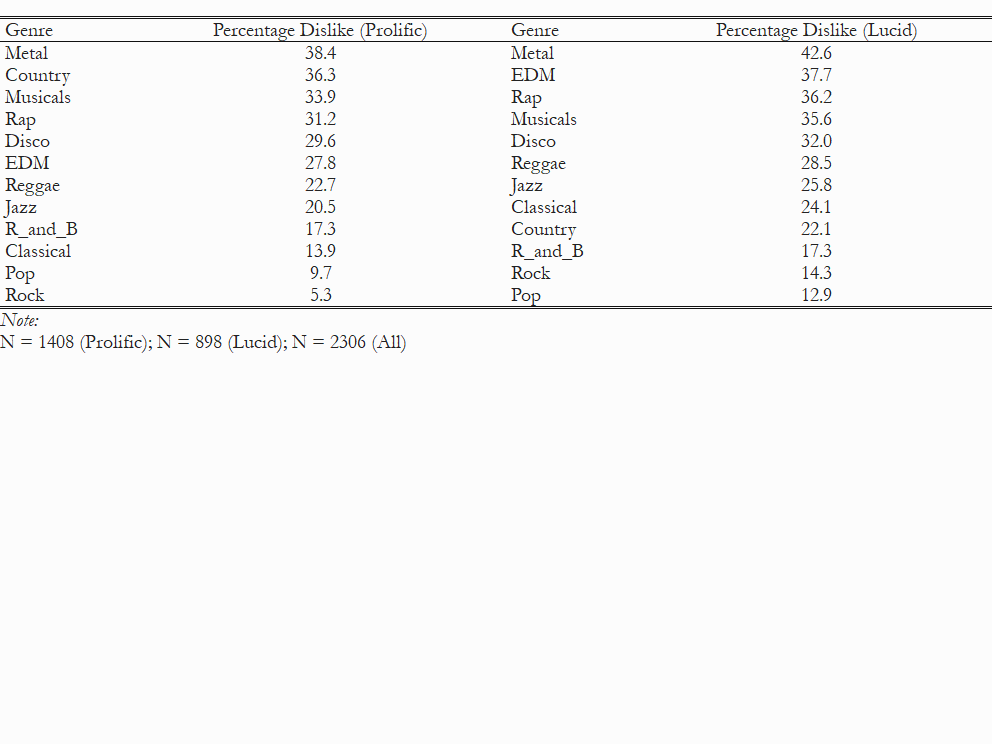
\includegraphics[trim={0 10cm 0 0},clip, width=1.0\textwidth]{Tabs/desc-tab-dislike.png}
    \label{tab:dis-by-genres}
\end{table}

\subsection*{Univariate Distribution of Number of Dislikes}
Table~\ref{tab:dis-dist} shows the univariate distribution of the number of dislikes for both the Prolific and Lucid samples. As we can see, both datasets agree closely in their estimate of the proportion of categorical tolerants, with the Prolific data returning an estimate of about 19\% of the sample and the Lucid dataset returning an estimate of about 20\%. When we combine both, we get an estimate of 19.6\%, suggesting that about a fifth of the American population today can be classified as categorical tolerants, an increase from L\&S's estimate of about 15\% using data from 2012.\footnote{We should be cautious when making direct comparisons, given that the number of genres included is smaller (twelve versus twenty in L\&S's 2012 survey) in both the Prolific and Lucid samples. Nevertheless, we can conclude that categorical tolerance remains a pervasive phenomenon among a substantial number of Americans.} 

\begin{table}[ht!]
    \caption{Univariate distribution of dislikes for the Prolific and Lucid samples.}
    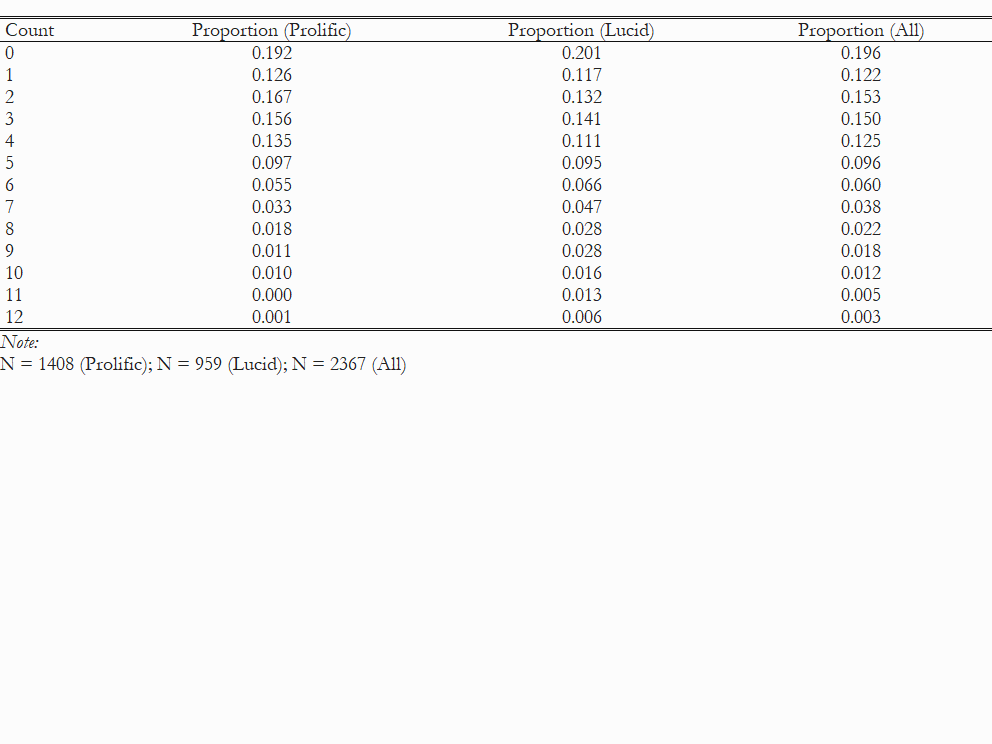
\includegraphics[trim={0 9.5cm 0 0},clip, width=1.0\textwidth]{Tabs/desc-tab-dislike-dist.png}
    \label{tab:dis-dist}
\end{table}

As shown in Figure~\ref{fig:main}, the distribution of the number of dislikes we get from the joint samples (like the separate sample distributions), exhibits excess zeroes, similar to the one obtained by L\&S using 2012 data. Even considering issues of sample comparability, we can conclude that the taste regime governing patterns of cultural choice among Americans in the second decade of the twenty-first century certainly no longer resembles that captured by the GSS in the early 1990s, with a larger-than-expected---if the number of dislikes followed a simple Poisson process---number of people refusing to express dislikes for any genre. 

\begin{figure}[ht!]
        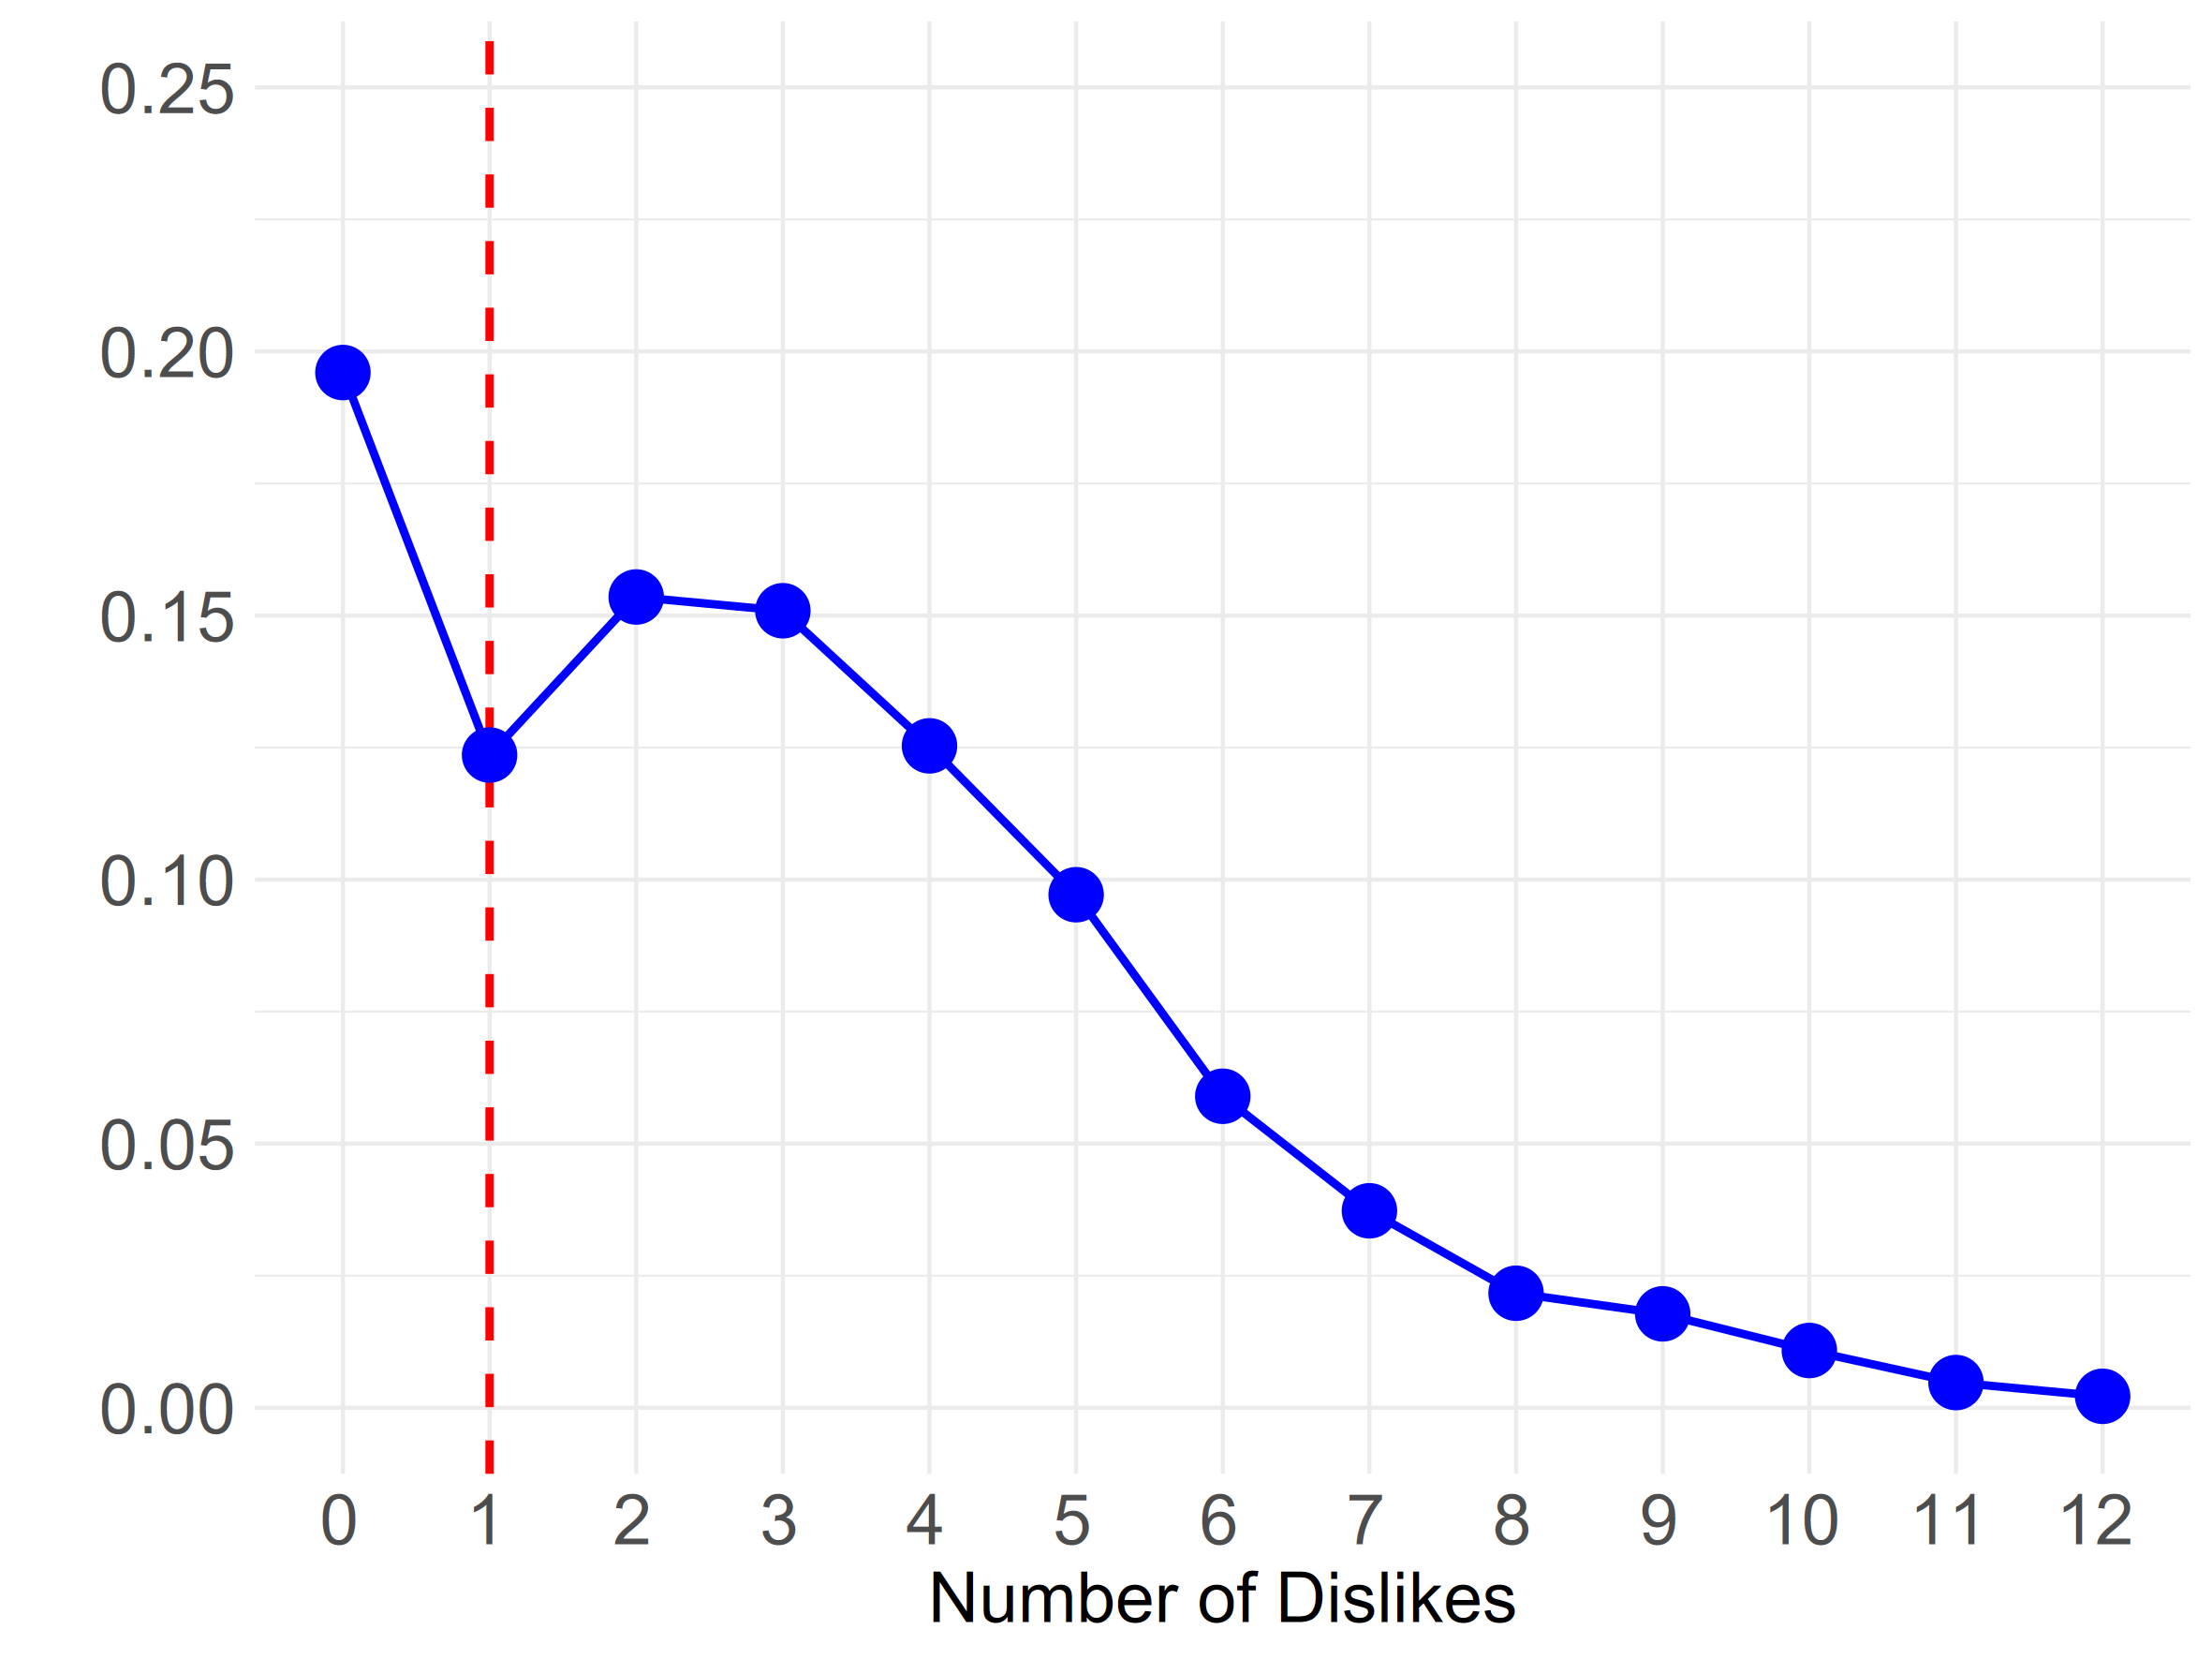
\includegraphics[width=1.0\textwidth]{Plots/uni-dist-cat-tol.png}
    \caption{Univariate plot of number of dislikes, joint Prolific and Lucid samples (N = 2306).}
    \label{fig:main}
\end{figure}

\subsection*{Socio-Demographic Distribution of Categorical Tolerance}
\begin{figure}[ht!]
    \captionsetup[subfigure]{font=footnotesize,labelfont=footnotesize}
    \centering
     \begin{subfigure}[b]{0.3\textwidth}
        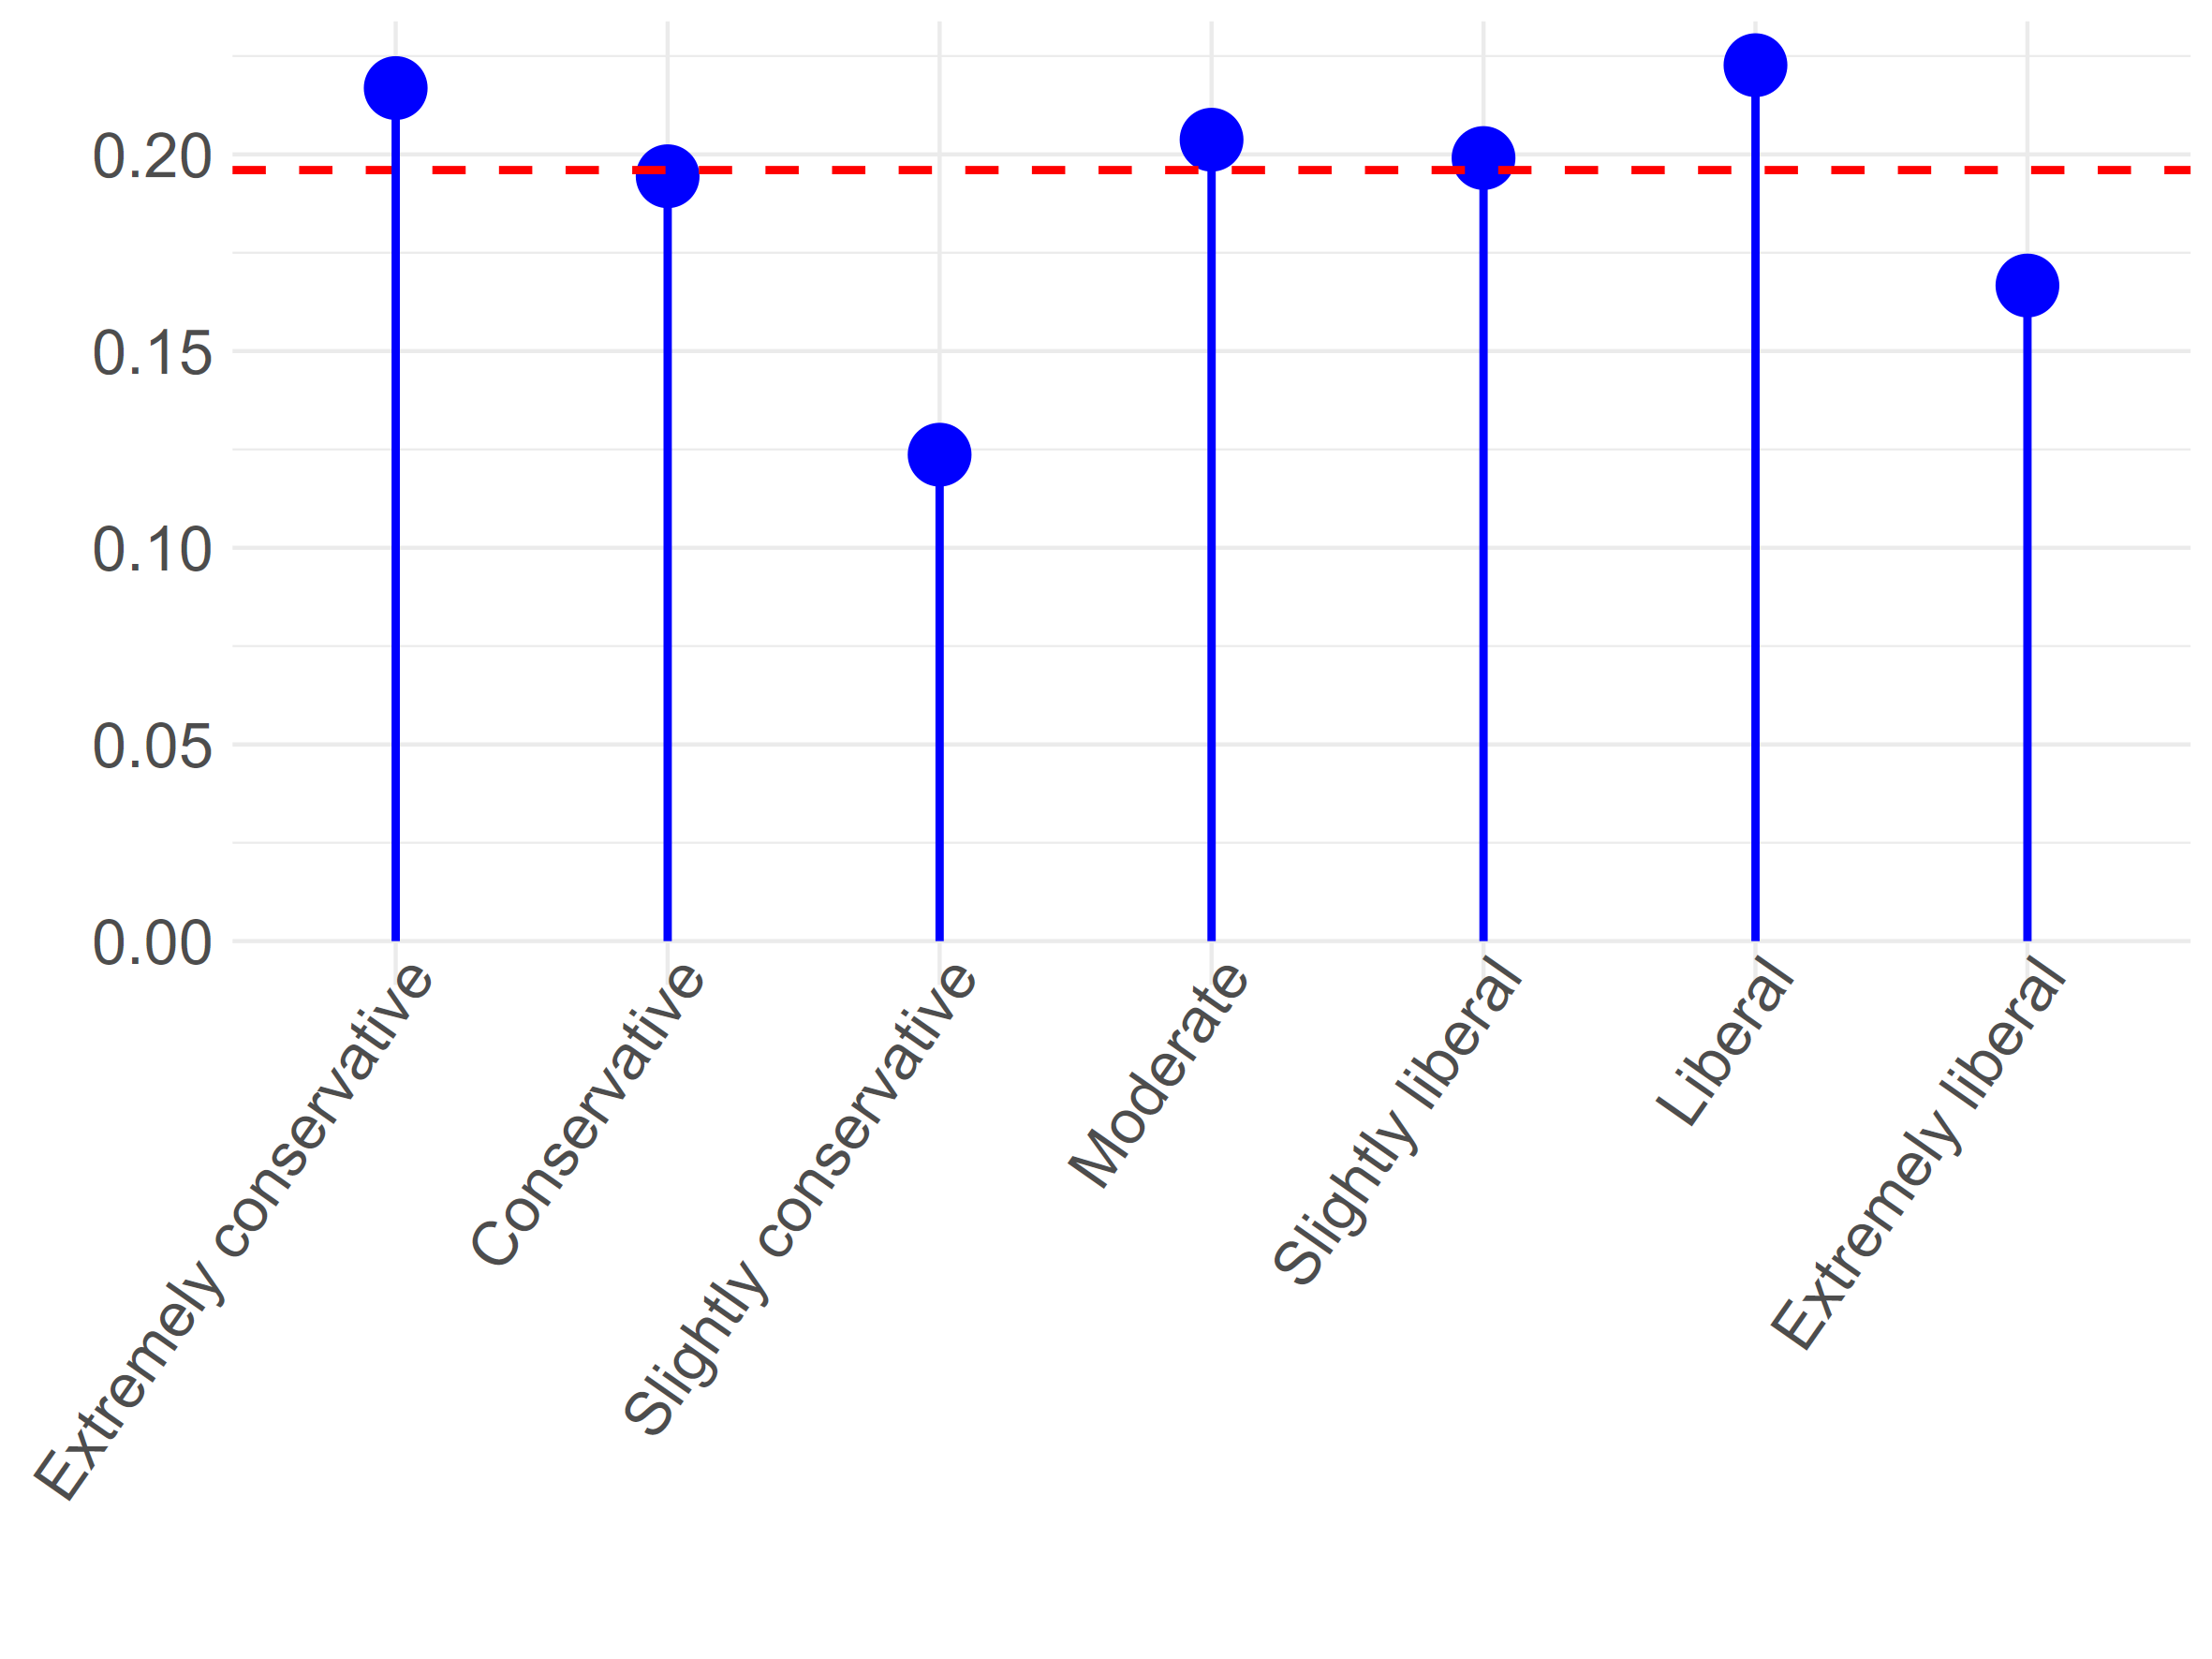
\includegraphics[width=1.0\textwidth]{Plots/uni-dist-cat-tol-pol.png}
            \caption{Political Ideology}
            \label{fig:cat-tol-pol}
    \end{subfigure}
     \begin{subfigure}[b]{0.3\textwidth}
        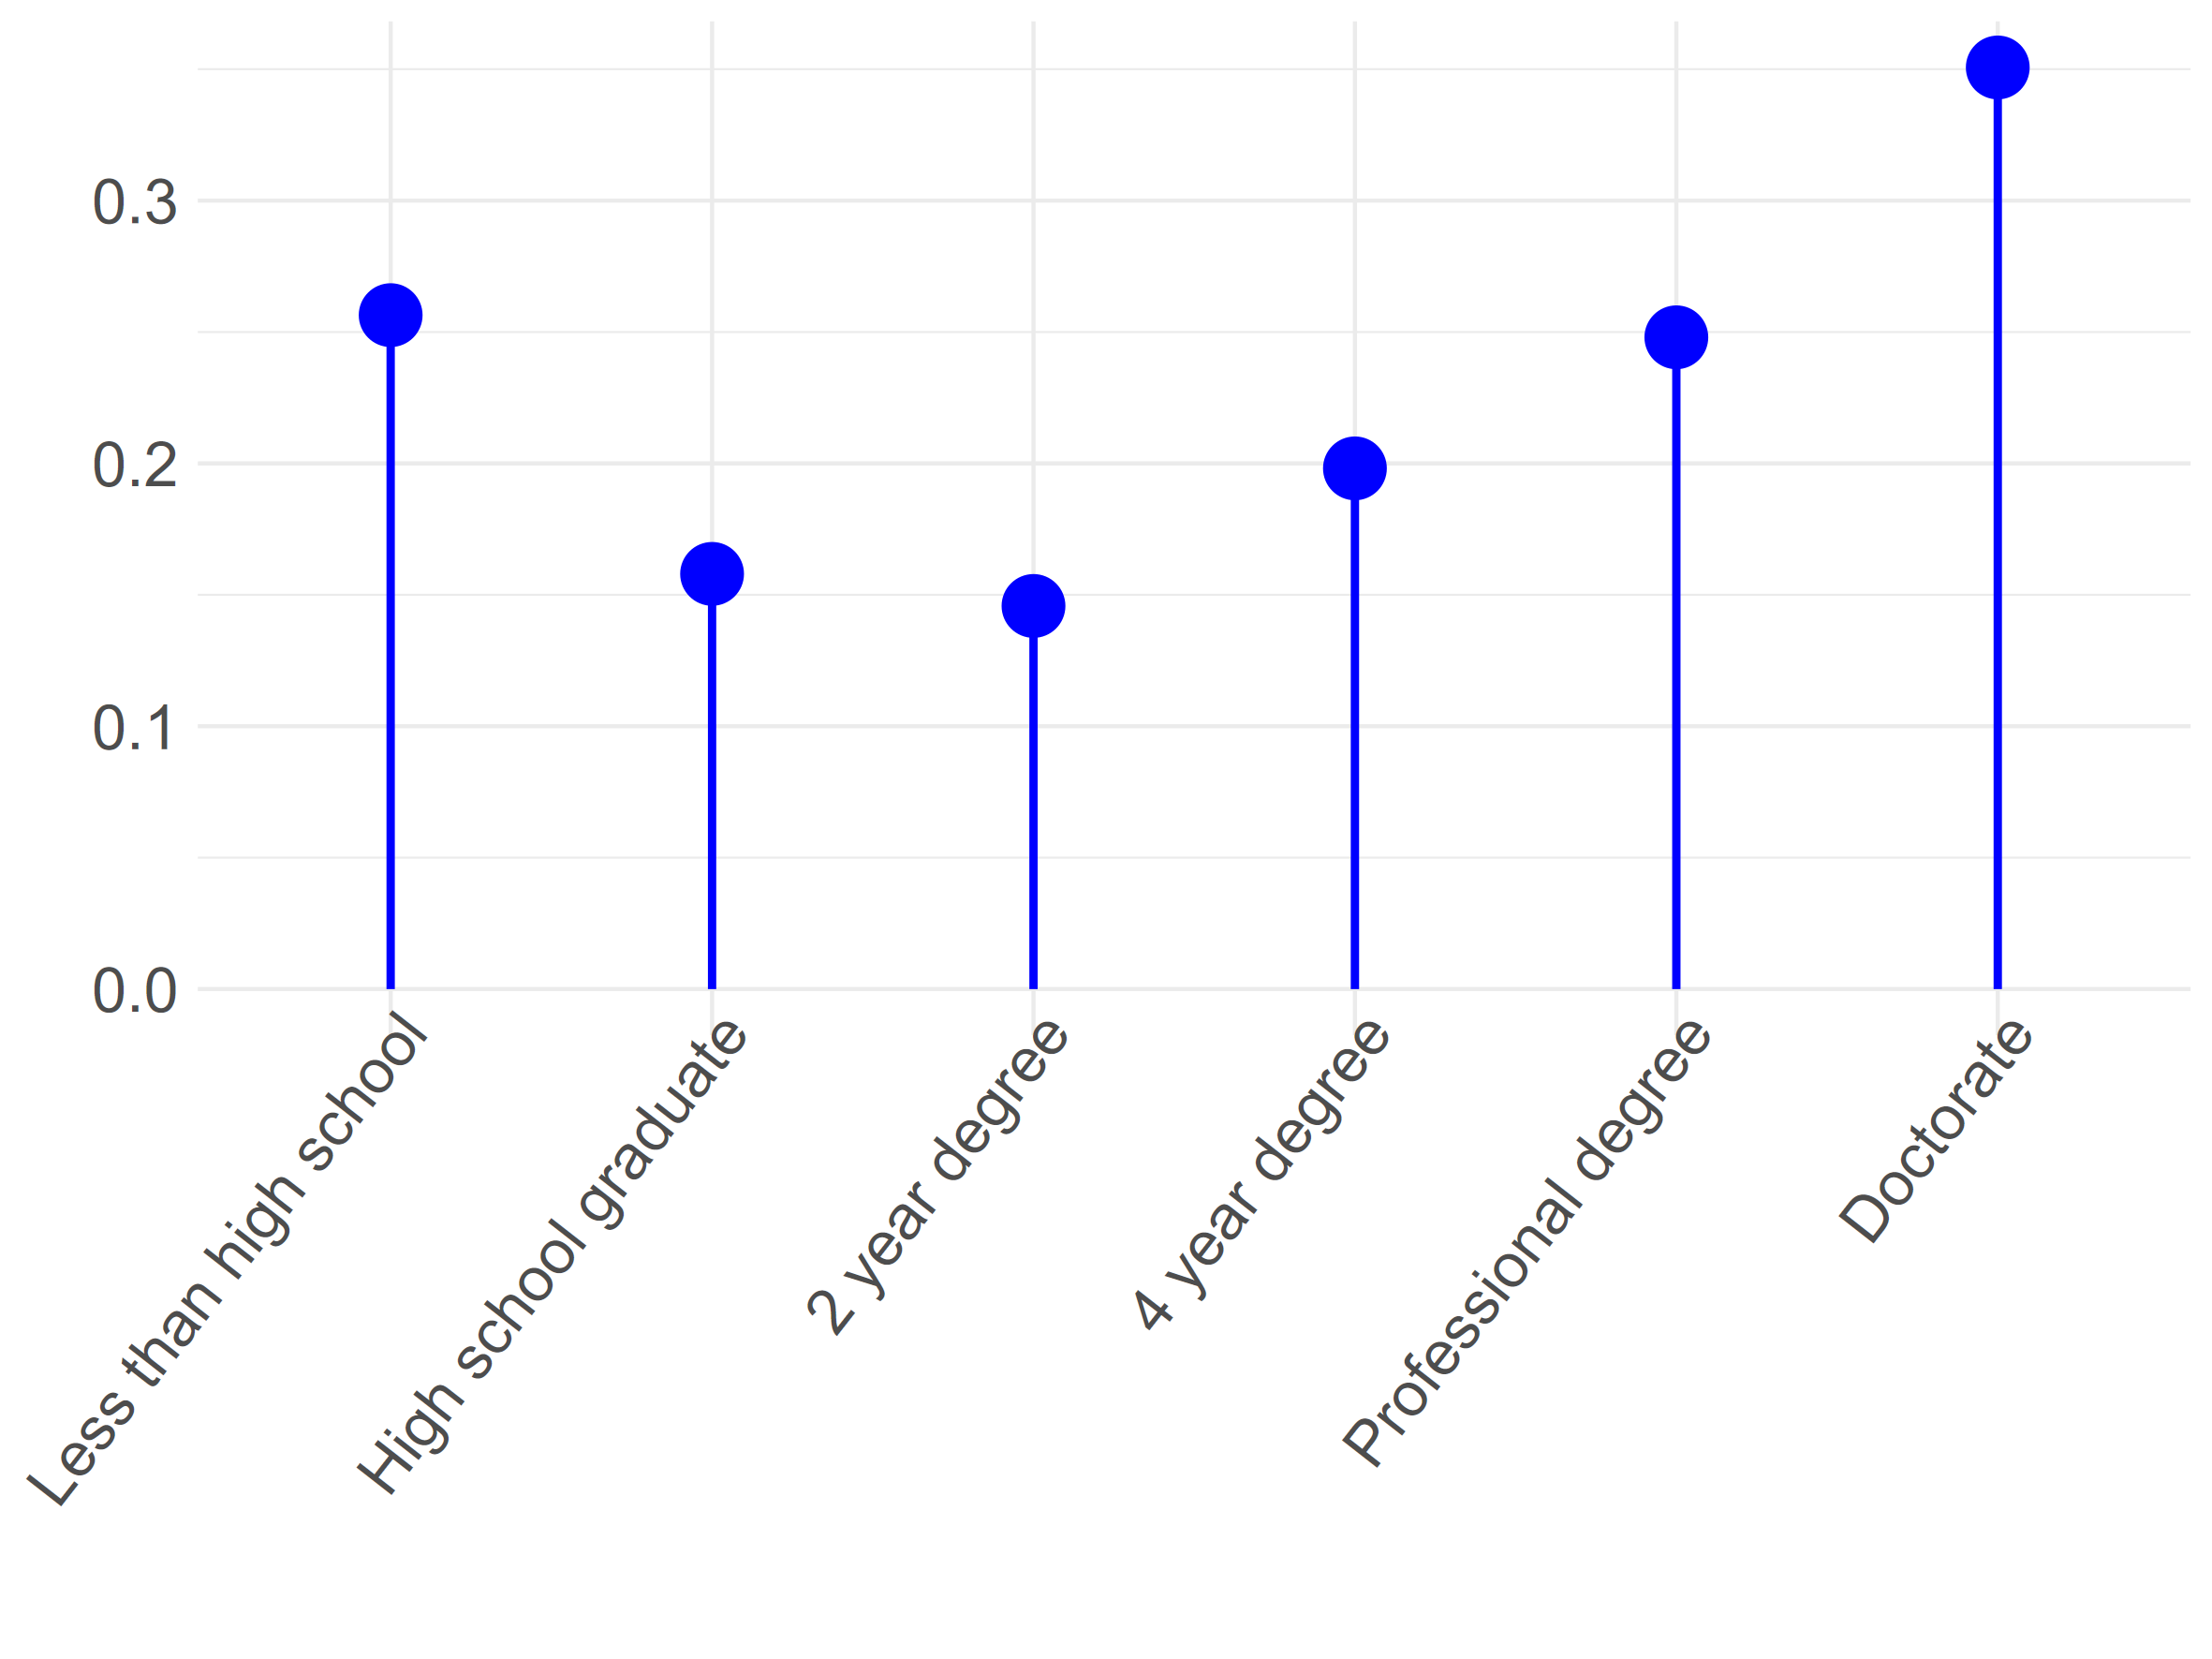
\includegraphics[width=1.0\textwidth]{Plots/uni-dist-cat-tol-edu.png}
            \caption{Education}
            \label{fig:cat-tol-edu}
    \end{subfigure}
     \begin{subfigure}[b]{0.3\textwidth}
        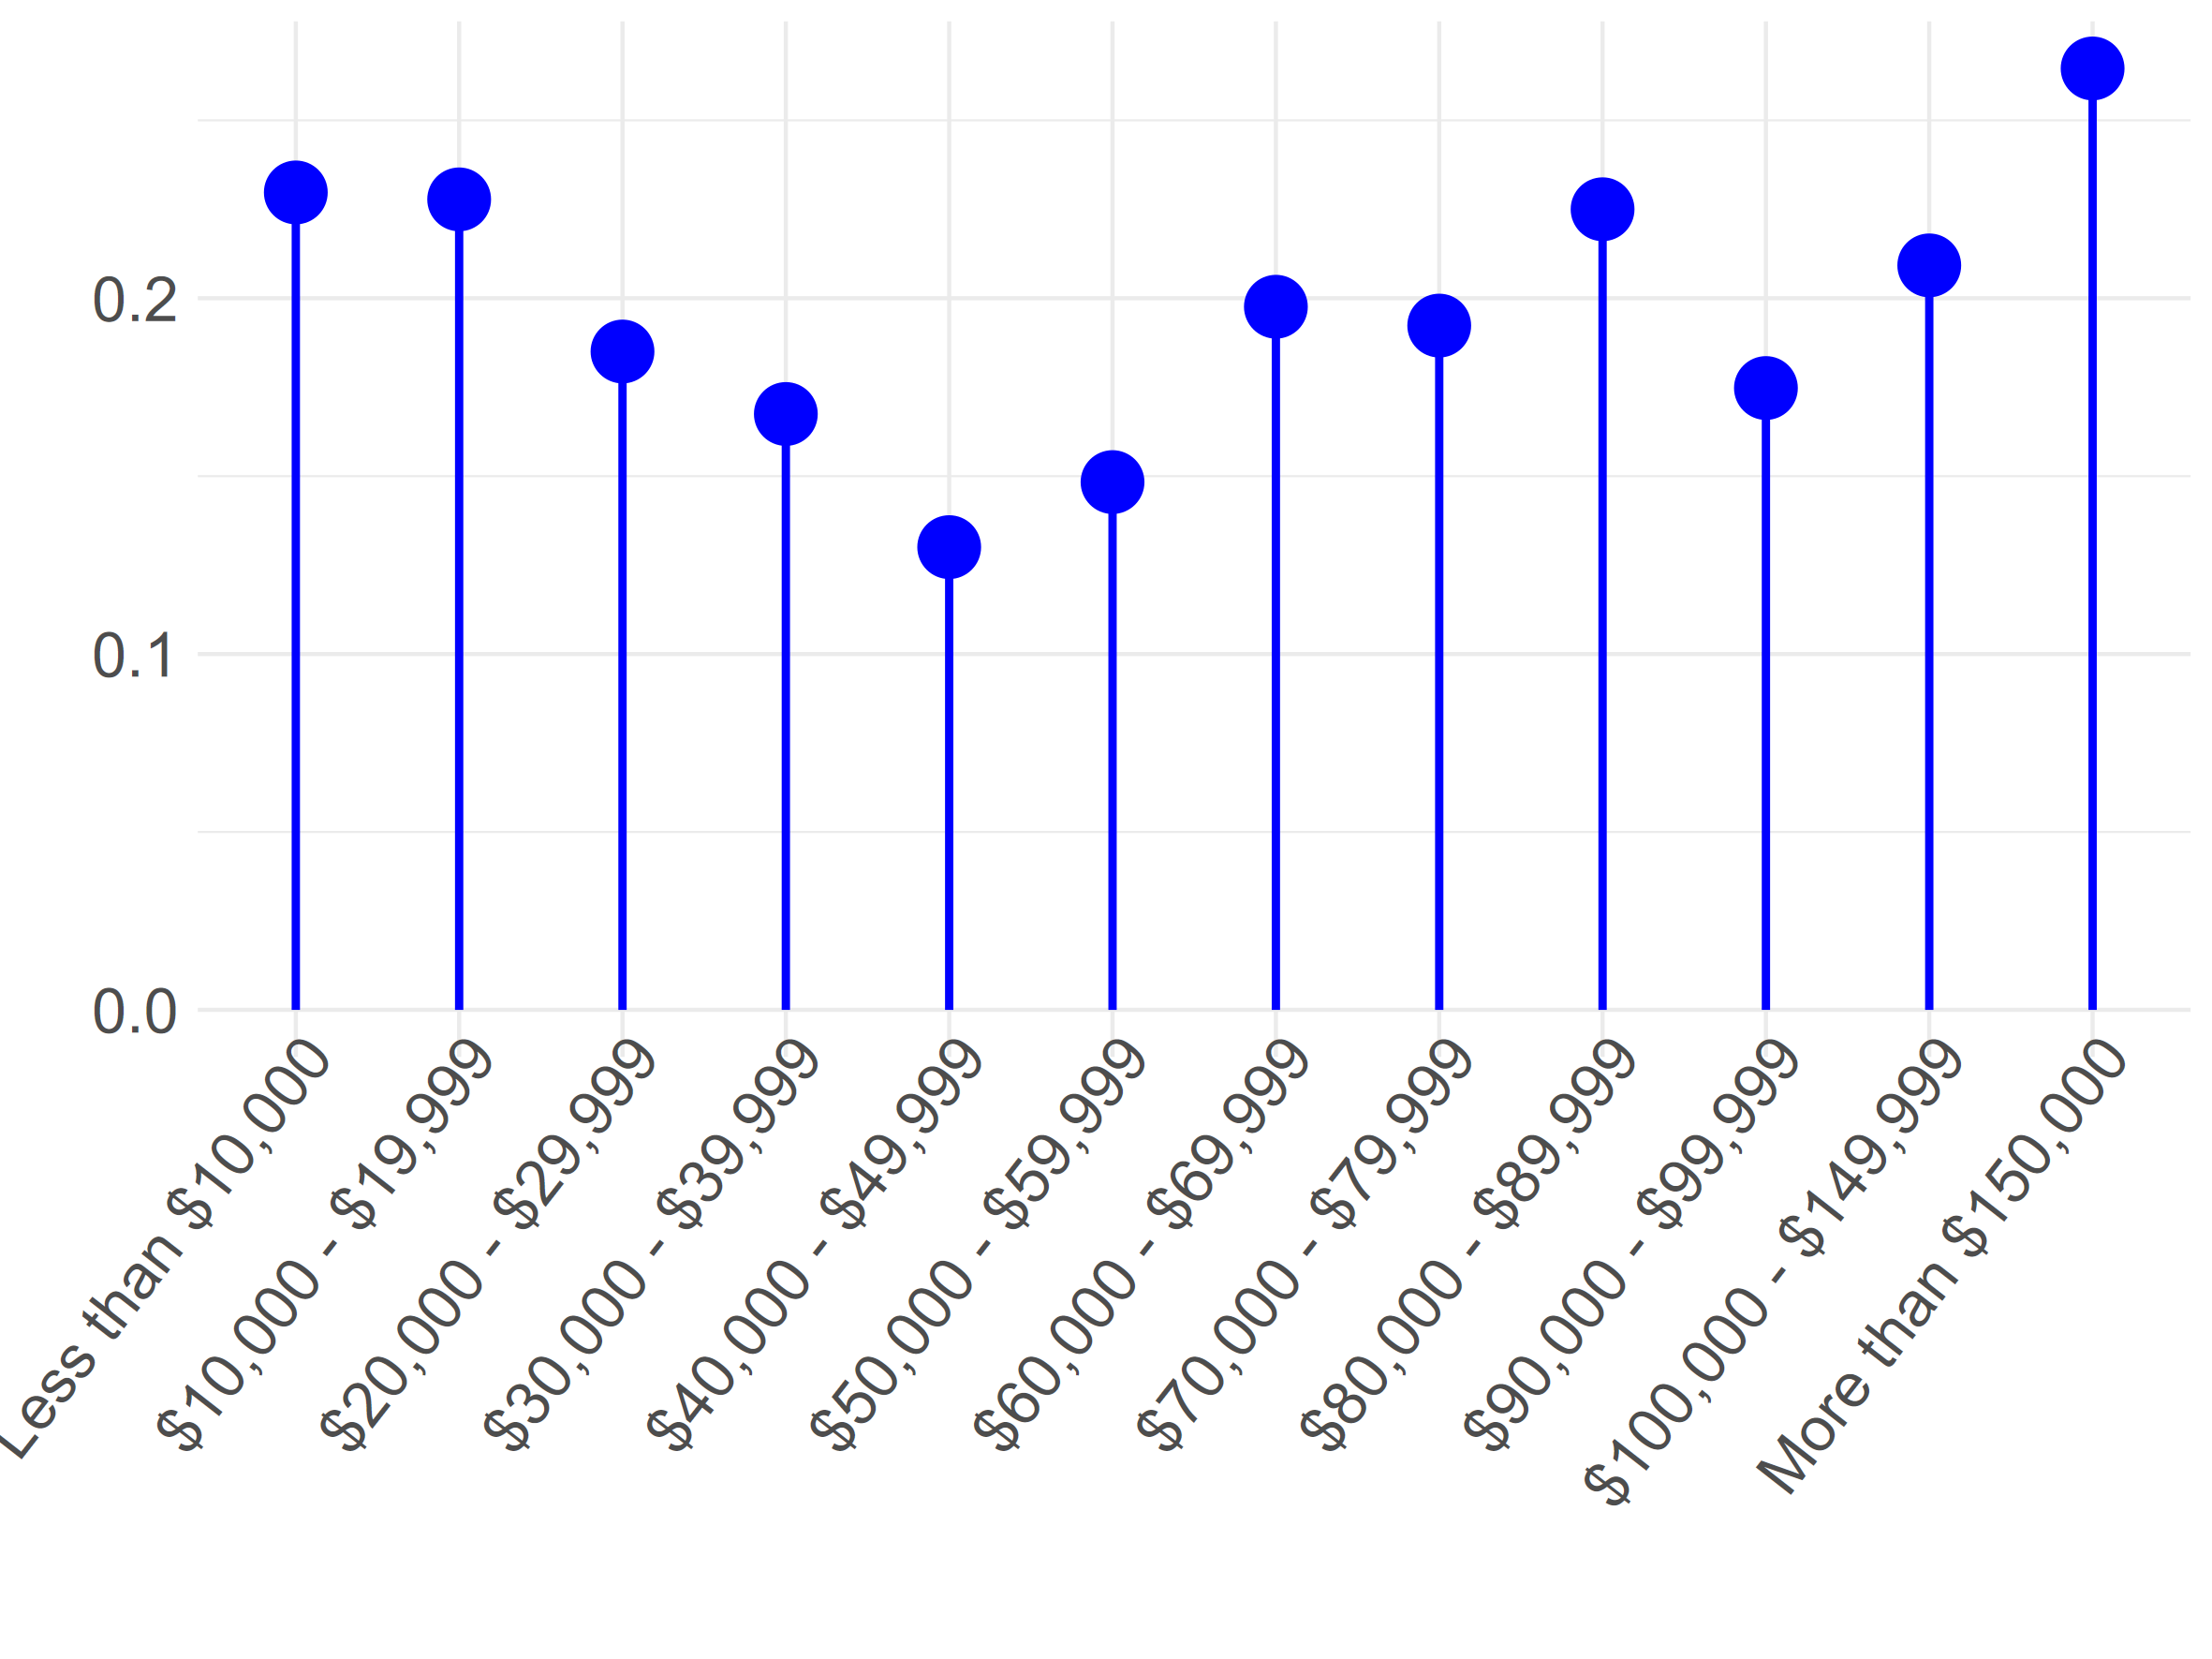
\includegraphics[width=1.0\textwidth]{Plots/uni-dist-cat-tol-inc.png}
            \caption{Income}
            \label{fig:cat-tol-inc}
    \end{subfigure}
     \begin{subfigure}[b]{0.3\textwidth}
        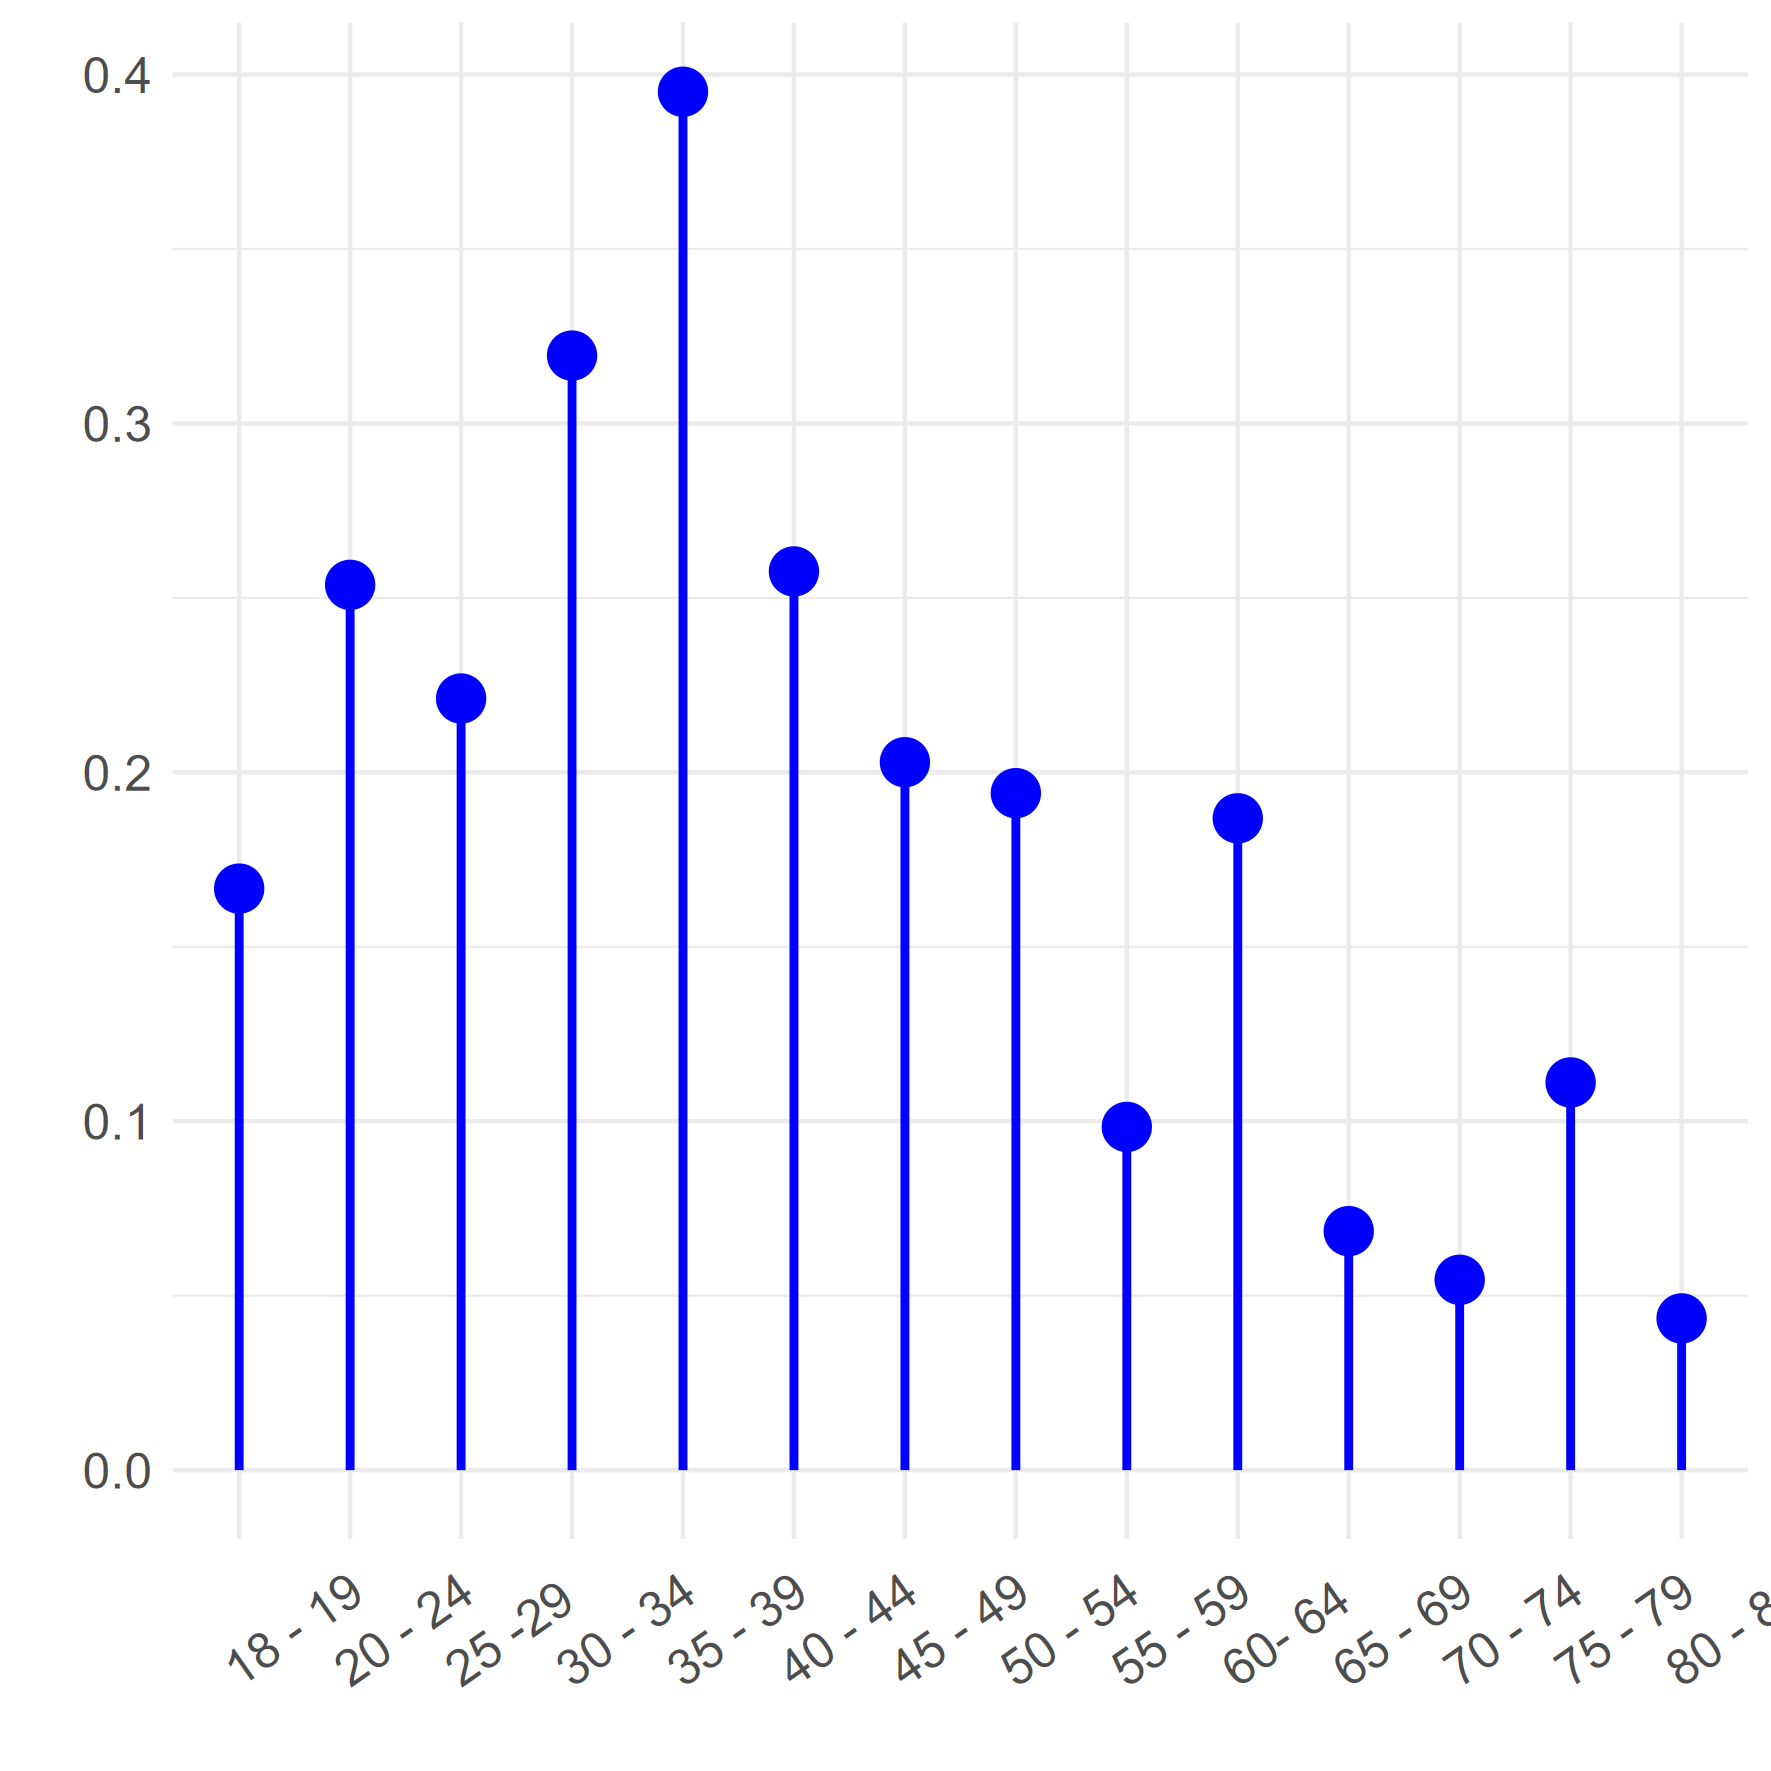
\includegraphics[width=1.0\textwidth]{Plots/uni-dist-cat-tol-age.png}
            \caption{Age}
            \label{fig:cat-tol-age}
    \end{subfigure}
     \begin{subfigure}[b]{0.3\textwidth}
        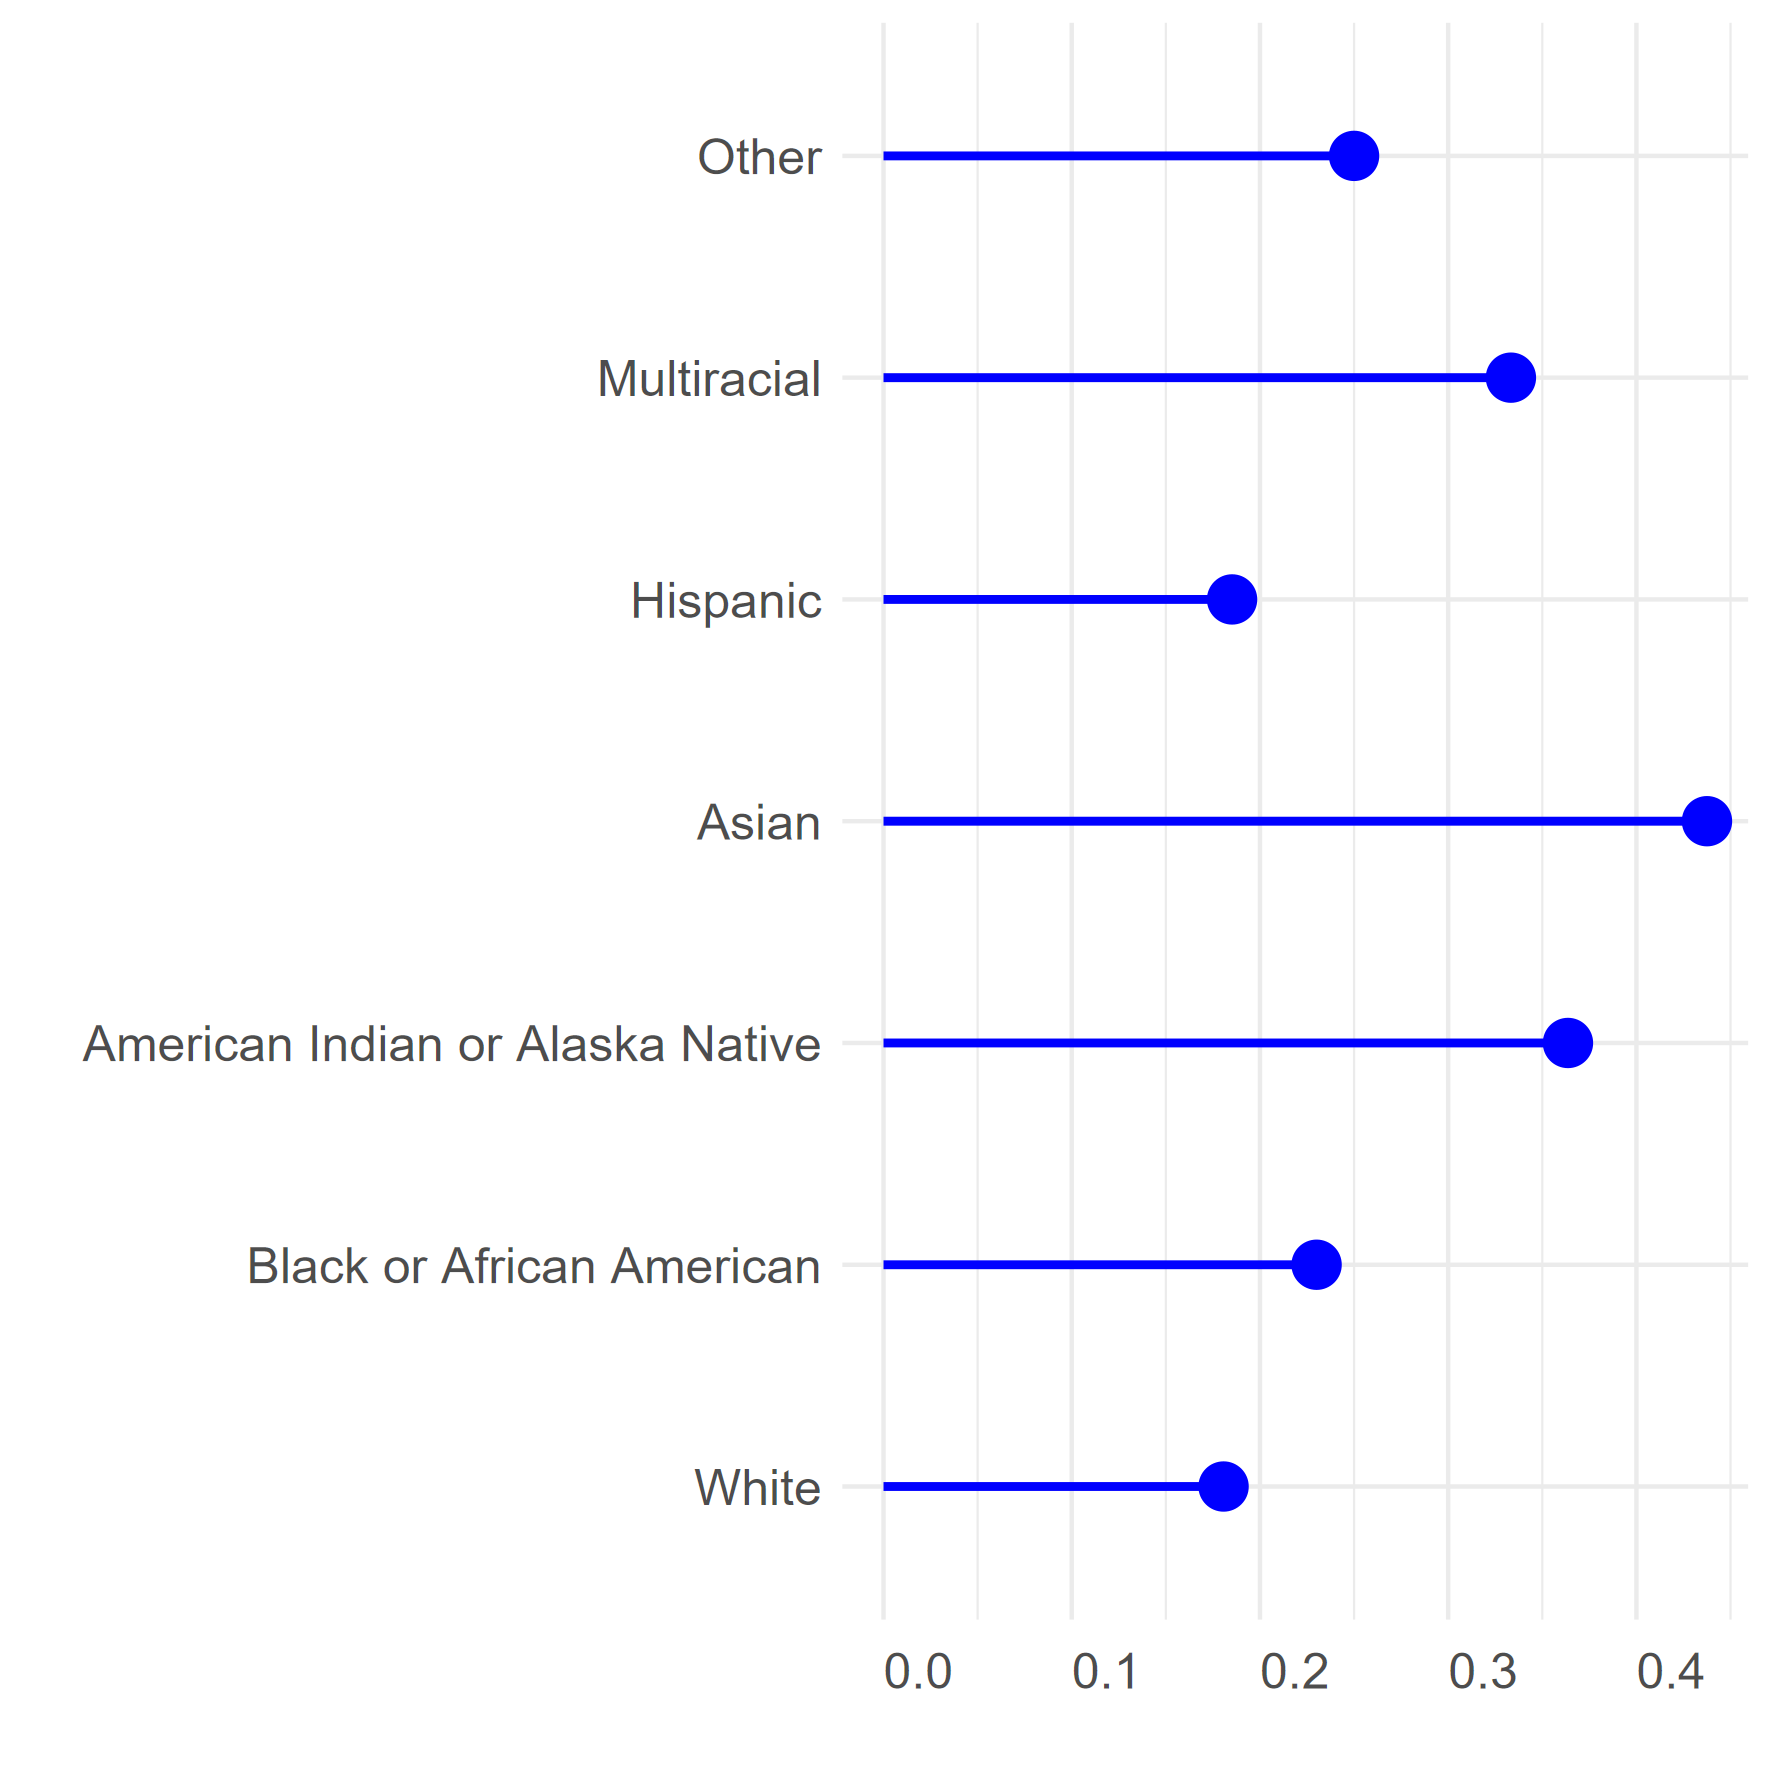
\includegraphics[width=1.0\textwidth]{Plots/uni-dist-cat-tol-rac.png}
            \caption{Ethnoracial Identification}
            \label{fig:cat-tol-rac}
    \end{subfigure}
     \begin{subfigure}[b]{0.3\textwidth}
        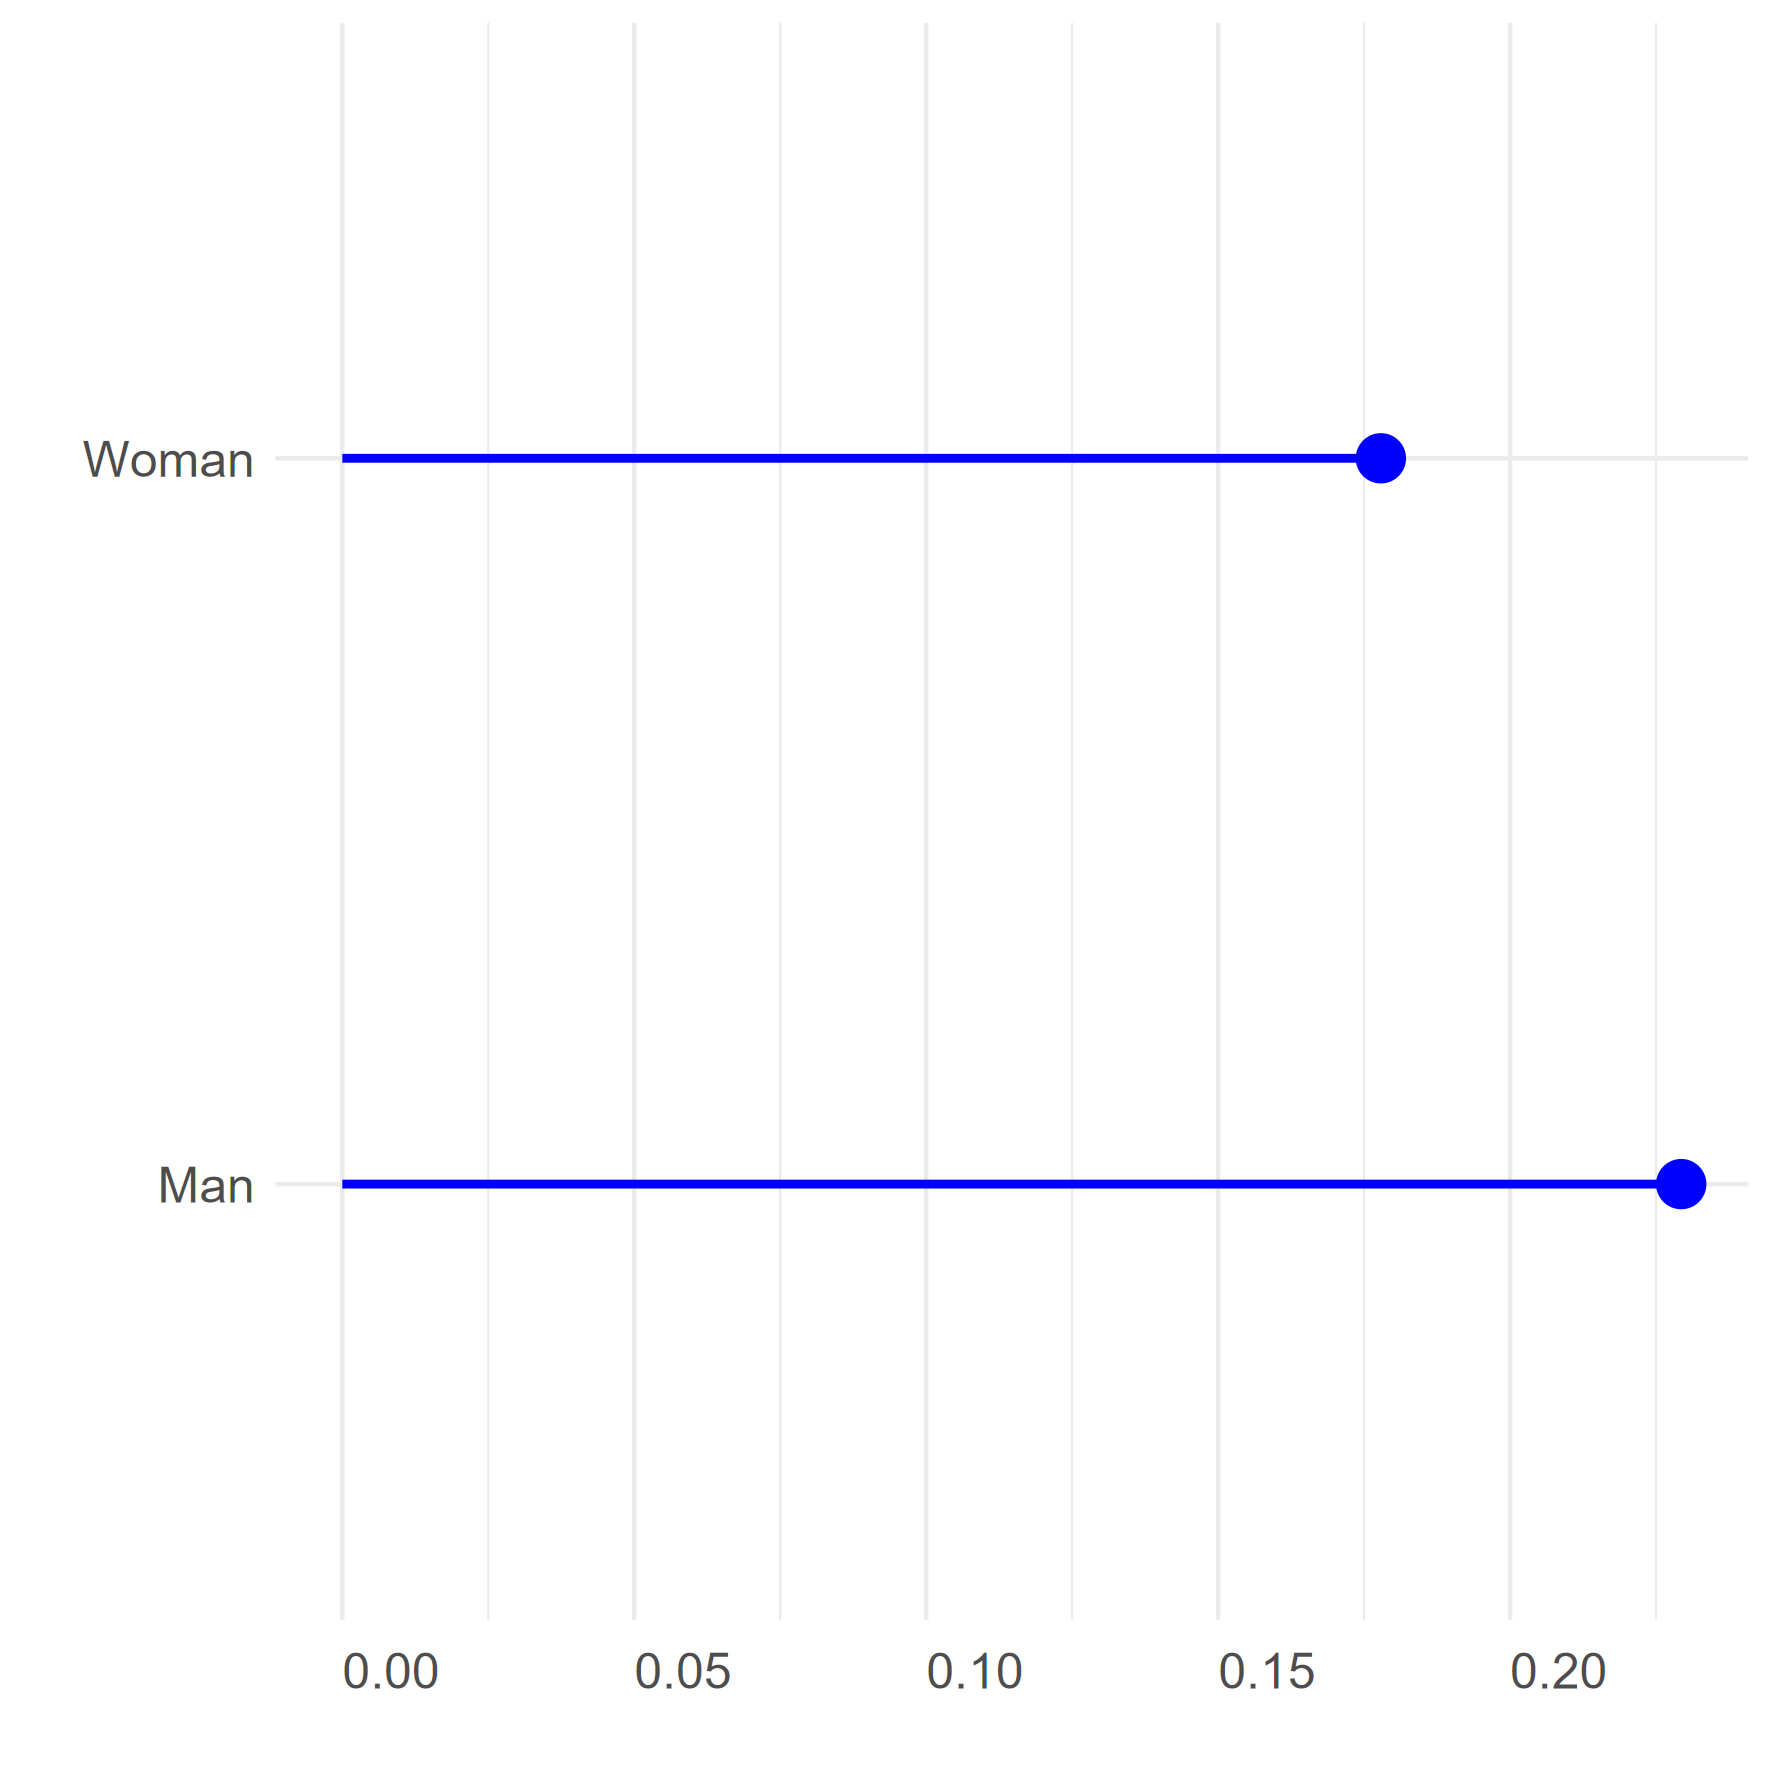
\includegraphics[width=1.0\textwidth]{Plots/uni-dist-cat-tol-gen.png}
            \caption{Gender Identification}
            \label{fig:cat-tol-gen}
    \end{subfigure}
    \caption{Proportion of Categorical Tolerants across different socio-demographic characteristics.}
    \label{fig:cat-tol}
\end{figure}

Figure~\ref{fig:cat-tol} shows how the sample probability of being a categorical tolerant is distributed among various socio-demographic categories. Each panel of Figure~\ref{fig:cat-tol} shows a ``lollipop plot'' with the numerical axis being the proportion of categorical tolerants at each level of the corresponding socio-demographic covariate. The red dashed reference line is the observed sample proportion of categorical tolerants. 

As Figure~\ref{fig:cat-tol-age} shows, age is the most straightforward factor structuring categorical tolerance, replicating the pattern observed by \citet{lizardo2016end-4fb}: Younger people are more likely to be categorical tolerants compared to older people, who are strongly under-represented among categorical tolerants; accordingly, the probability of being a categorical tolerant in these data is maximized among younger adults (individuals in their thirties), suggesting that very young people are induced to use musical genres for purposes of symbolic inclusion to a greater extent than people at this life-stage. Regardless, it is clear that if cohort replacement dynamics drive the rise of categorical tolerance, then we should expect it to remain a fixture of the cultural taste landscape in the U.S. as older, less categorically tolerant cohorts exit the population. 

The other obvious factor structuring categorical tolerance in the United States is race. Mirroring L\&S's earlier findings, Figure~\ref{fig:cat-tol-rac} shows that categorical tolerance continues to be primarily a non-white phenomenon, with whites (and to a similar extent respondents who identify as Hispanic) under-represented among categorical tolerants, and Black, Asian, and Native American respondents over-represented. Also similar to L\&S's findings, the traditional Bourdieusian structuring factors (e.g., education and income) do not have a straightforward link to categorical tolerance, with both showing non-linear patterns (categorical tolerants over-represented among both high and low education and high and low-income respondents). 

Nevertheless, the apparent over-representation of the most highly educated stratum among the categorically tolerant suggests an elite move in this direction, which was not evident in L\&S's previous analysis, which mainly pointed to cohort/age and ethnoracial status effects. Interestingly, we also observe a strong gender effect---unlike L\&S's earlier findings---which suggests a relatively large gender gap in the categorical tolerance taste pattern, with men overrepresented and women underrepresented among the ranks of categorical tolerants. Finally, categorical tolerance---in contrast to symbolic exclusion as we will see in a bit---is not polarized along political-ideological lines, with no clear pattern shown according to conservative/liberal placement. 

\subsection*{Socio-Demographic Distribution of Symbolic Exclusion}
The obverse phenomenon of categorical tolerance is \emph{symbolic exclusion} \citep{bryson1996anything-311}, that is, the probability of expressing at least one dislike, among those in the population who are at risk of doing so. Figure~\ref{fig:grd-int} shows the distribution of symbolic exclusion propensities in the joint Prolific and Lucid sample using a similar plotting strategy as Figure~\ref{fig:cat-tol}, but this time with the average number of dislikes expressed by members of each socio-demographic category in the numerical axis. The dashed red reference line, like before, represents the average number of dislikes among individuals in the joint sample. 

\begin{figure}[ht!]
    \captionsetup[subfigure]{font=footnotesize,labelfont=footnotesize}
    \centering
     \begin{subfigure}[b]{0.3\textwidth}
        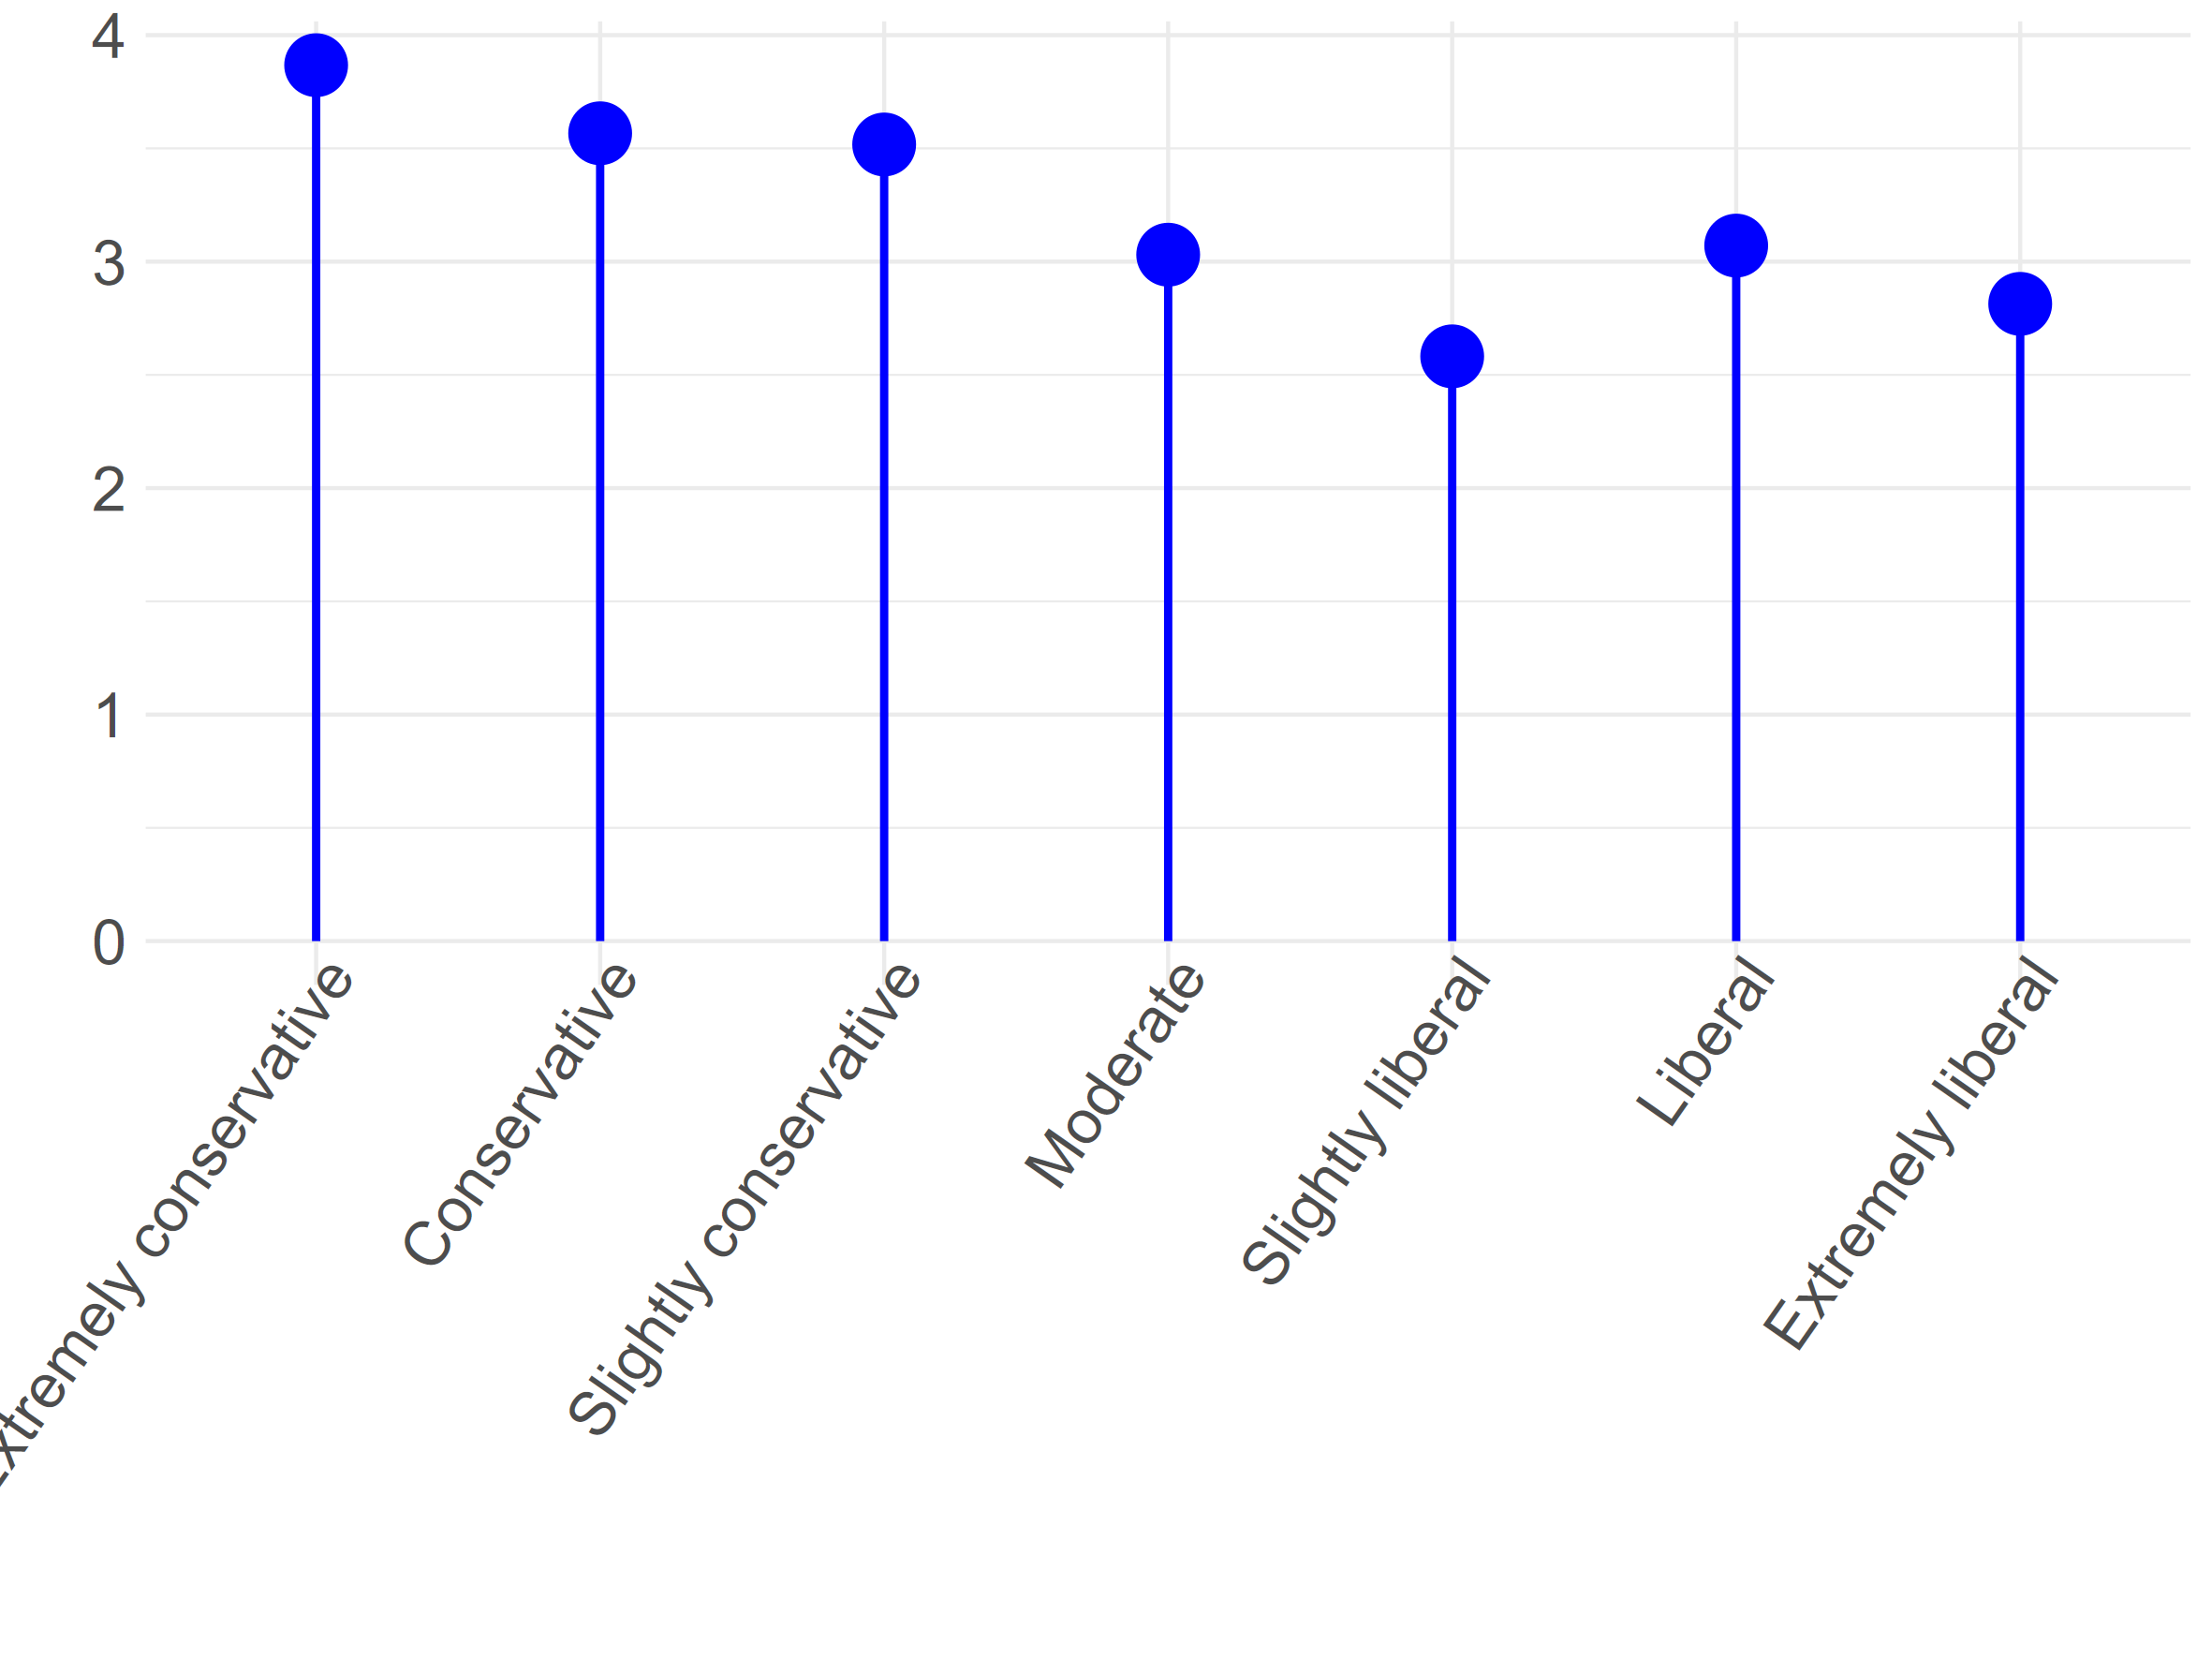
\includegraphics[width=1.0\textwidth]{Plots/uni-dist-grd-int-pol.png}
            \caption{Political Ideology}
            \label{fig:grd-int-pol}
    \end{subfigure}
     \begin{subfigure}[b]{0.3\textwidth}
        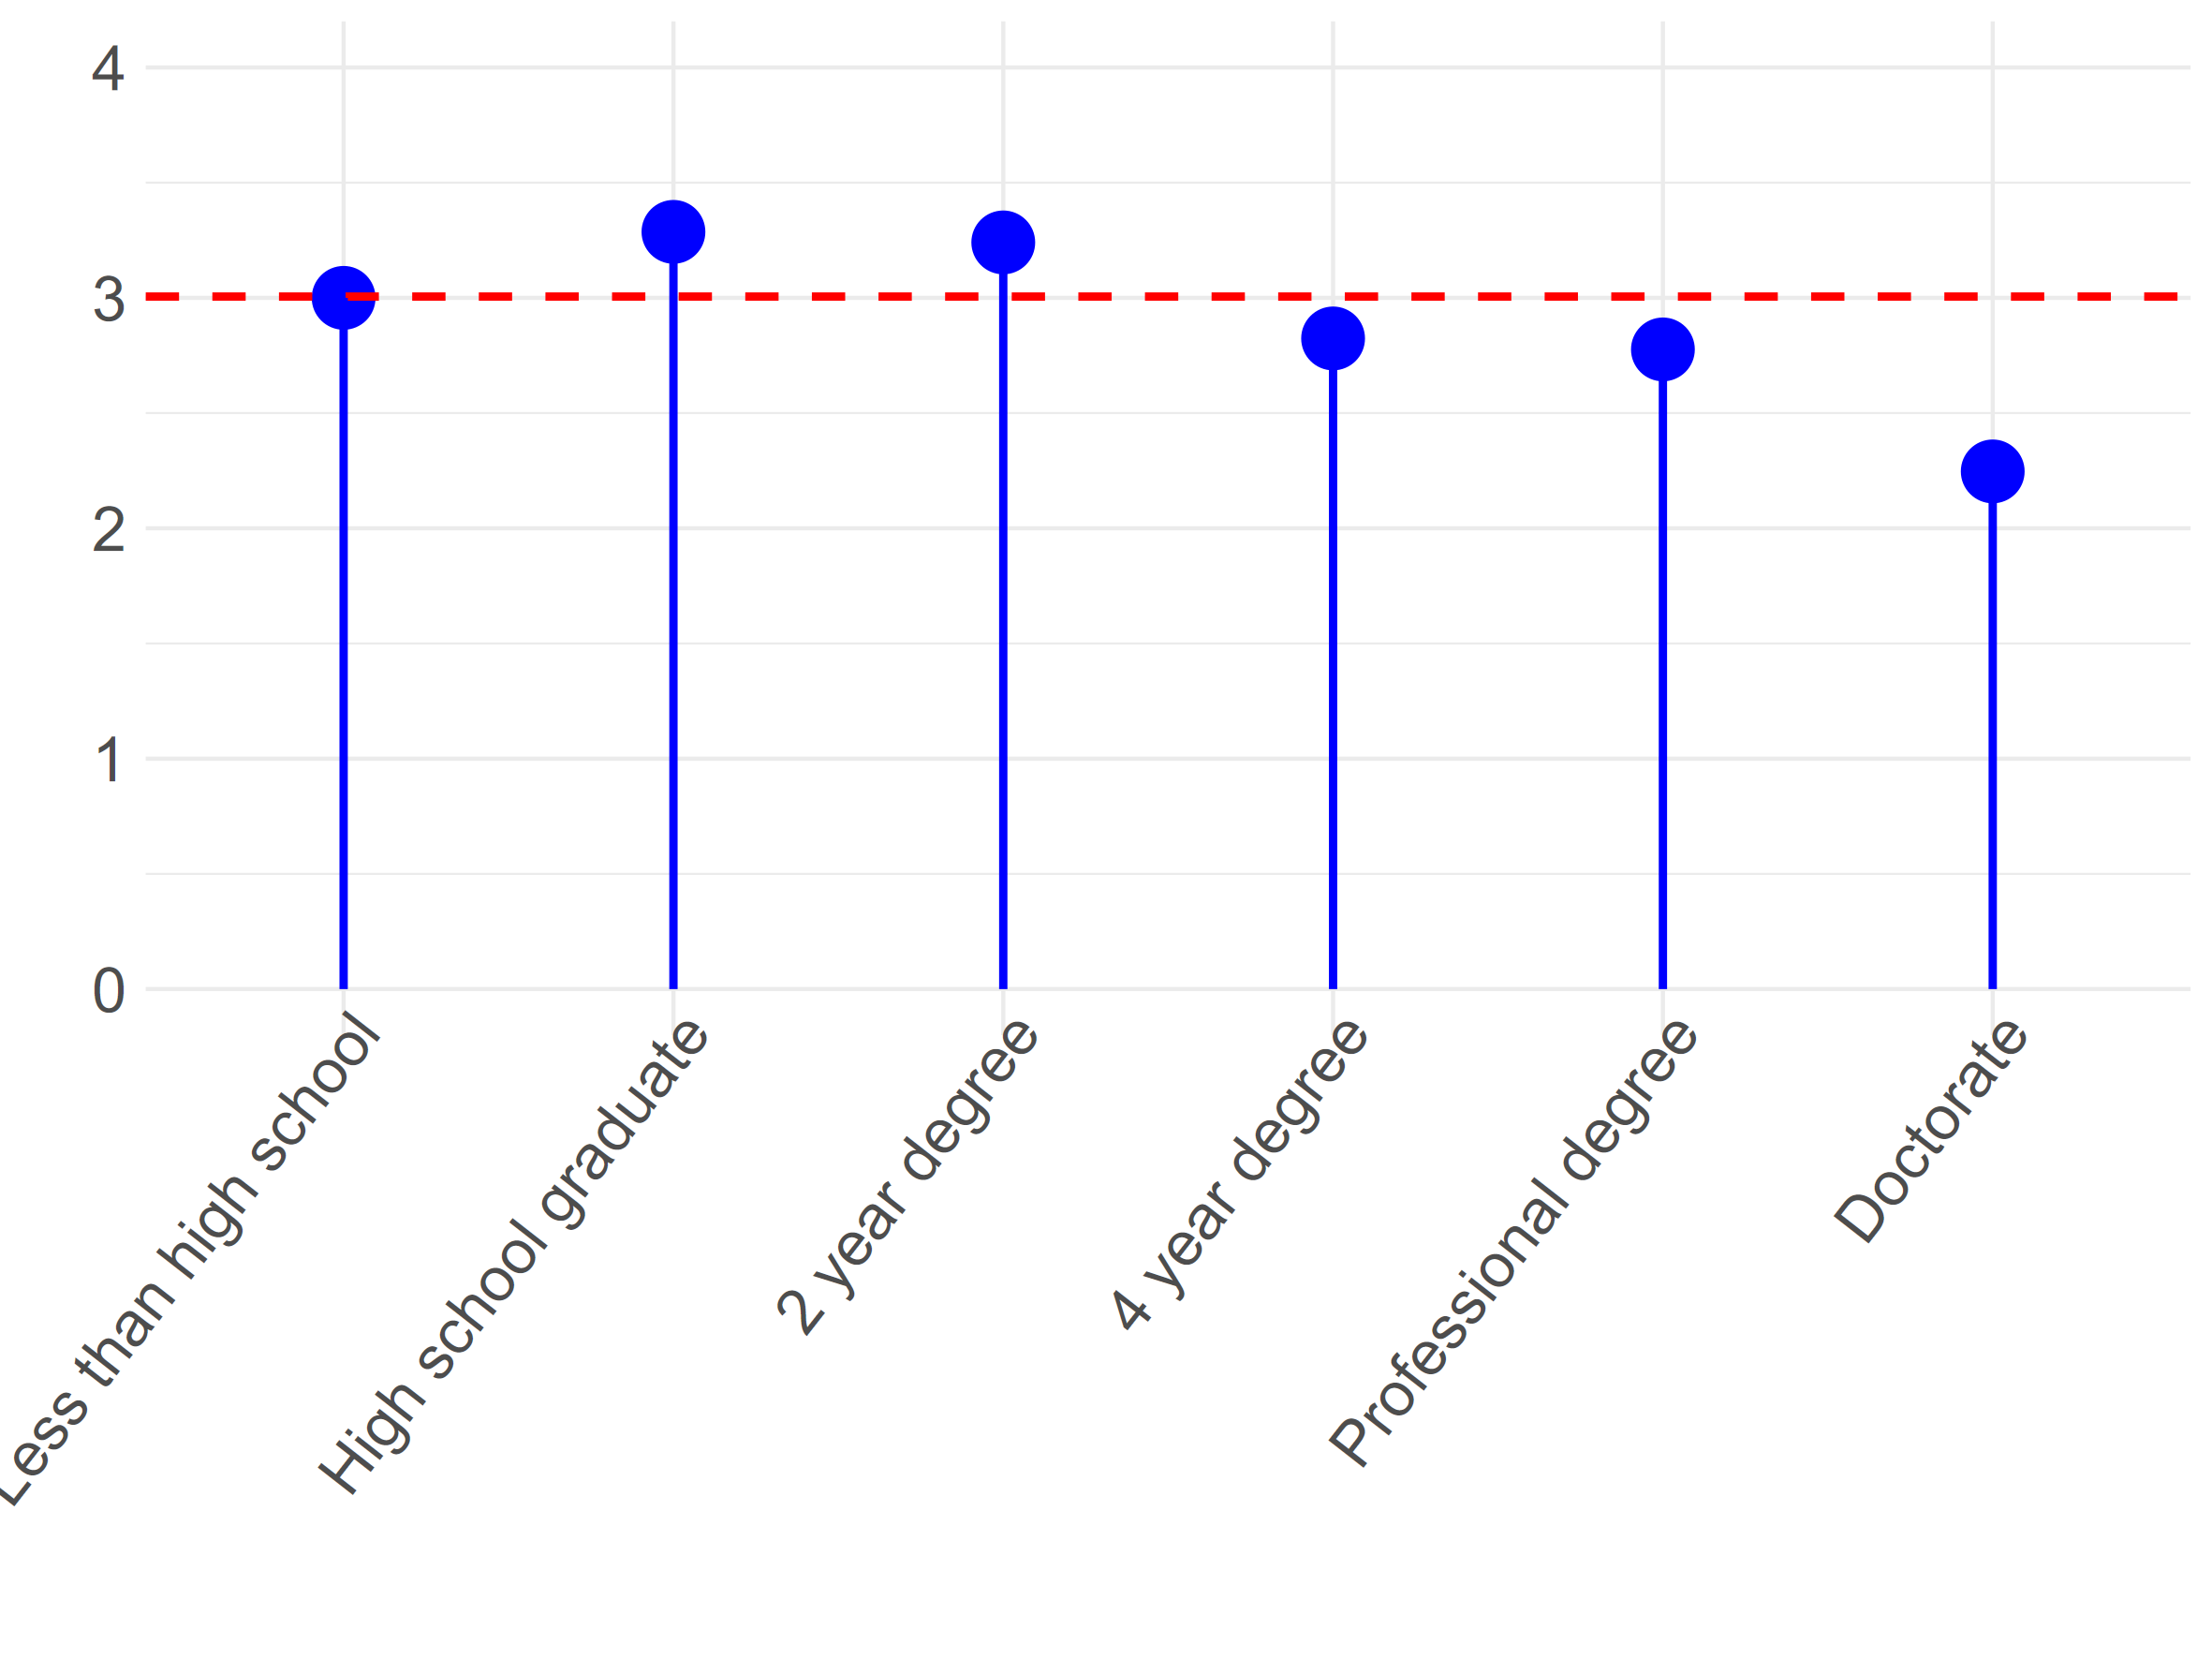
\includegraphics[width=1.0\textwidth]{Plots/uni-dist-grd-int-edu.png}
            \caption{Education}
            \label{fig:grd-int-edu}
    \end{subfigure}
     \begin{subfigure}[b]{0.3\textwidth}
        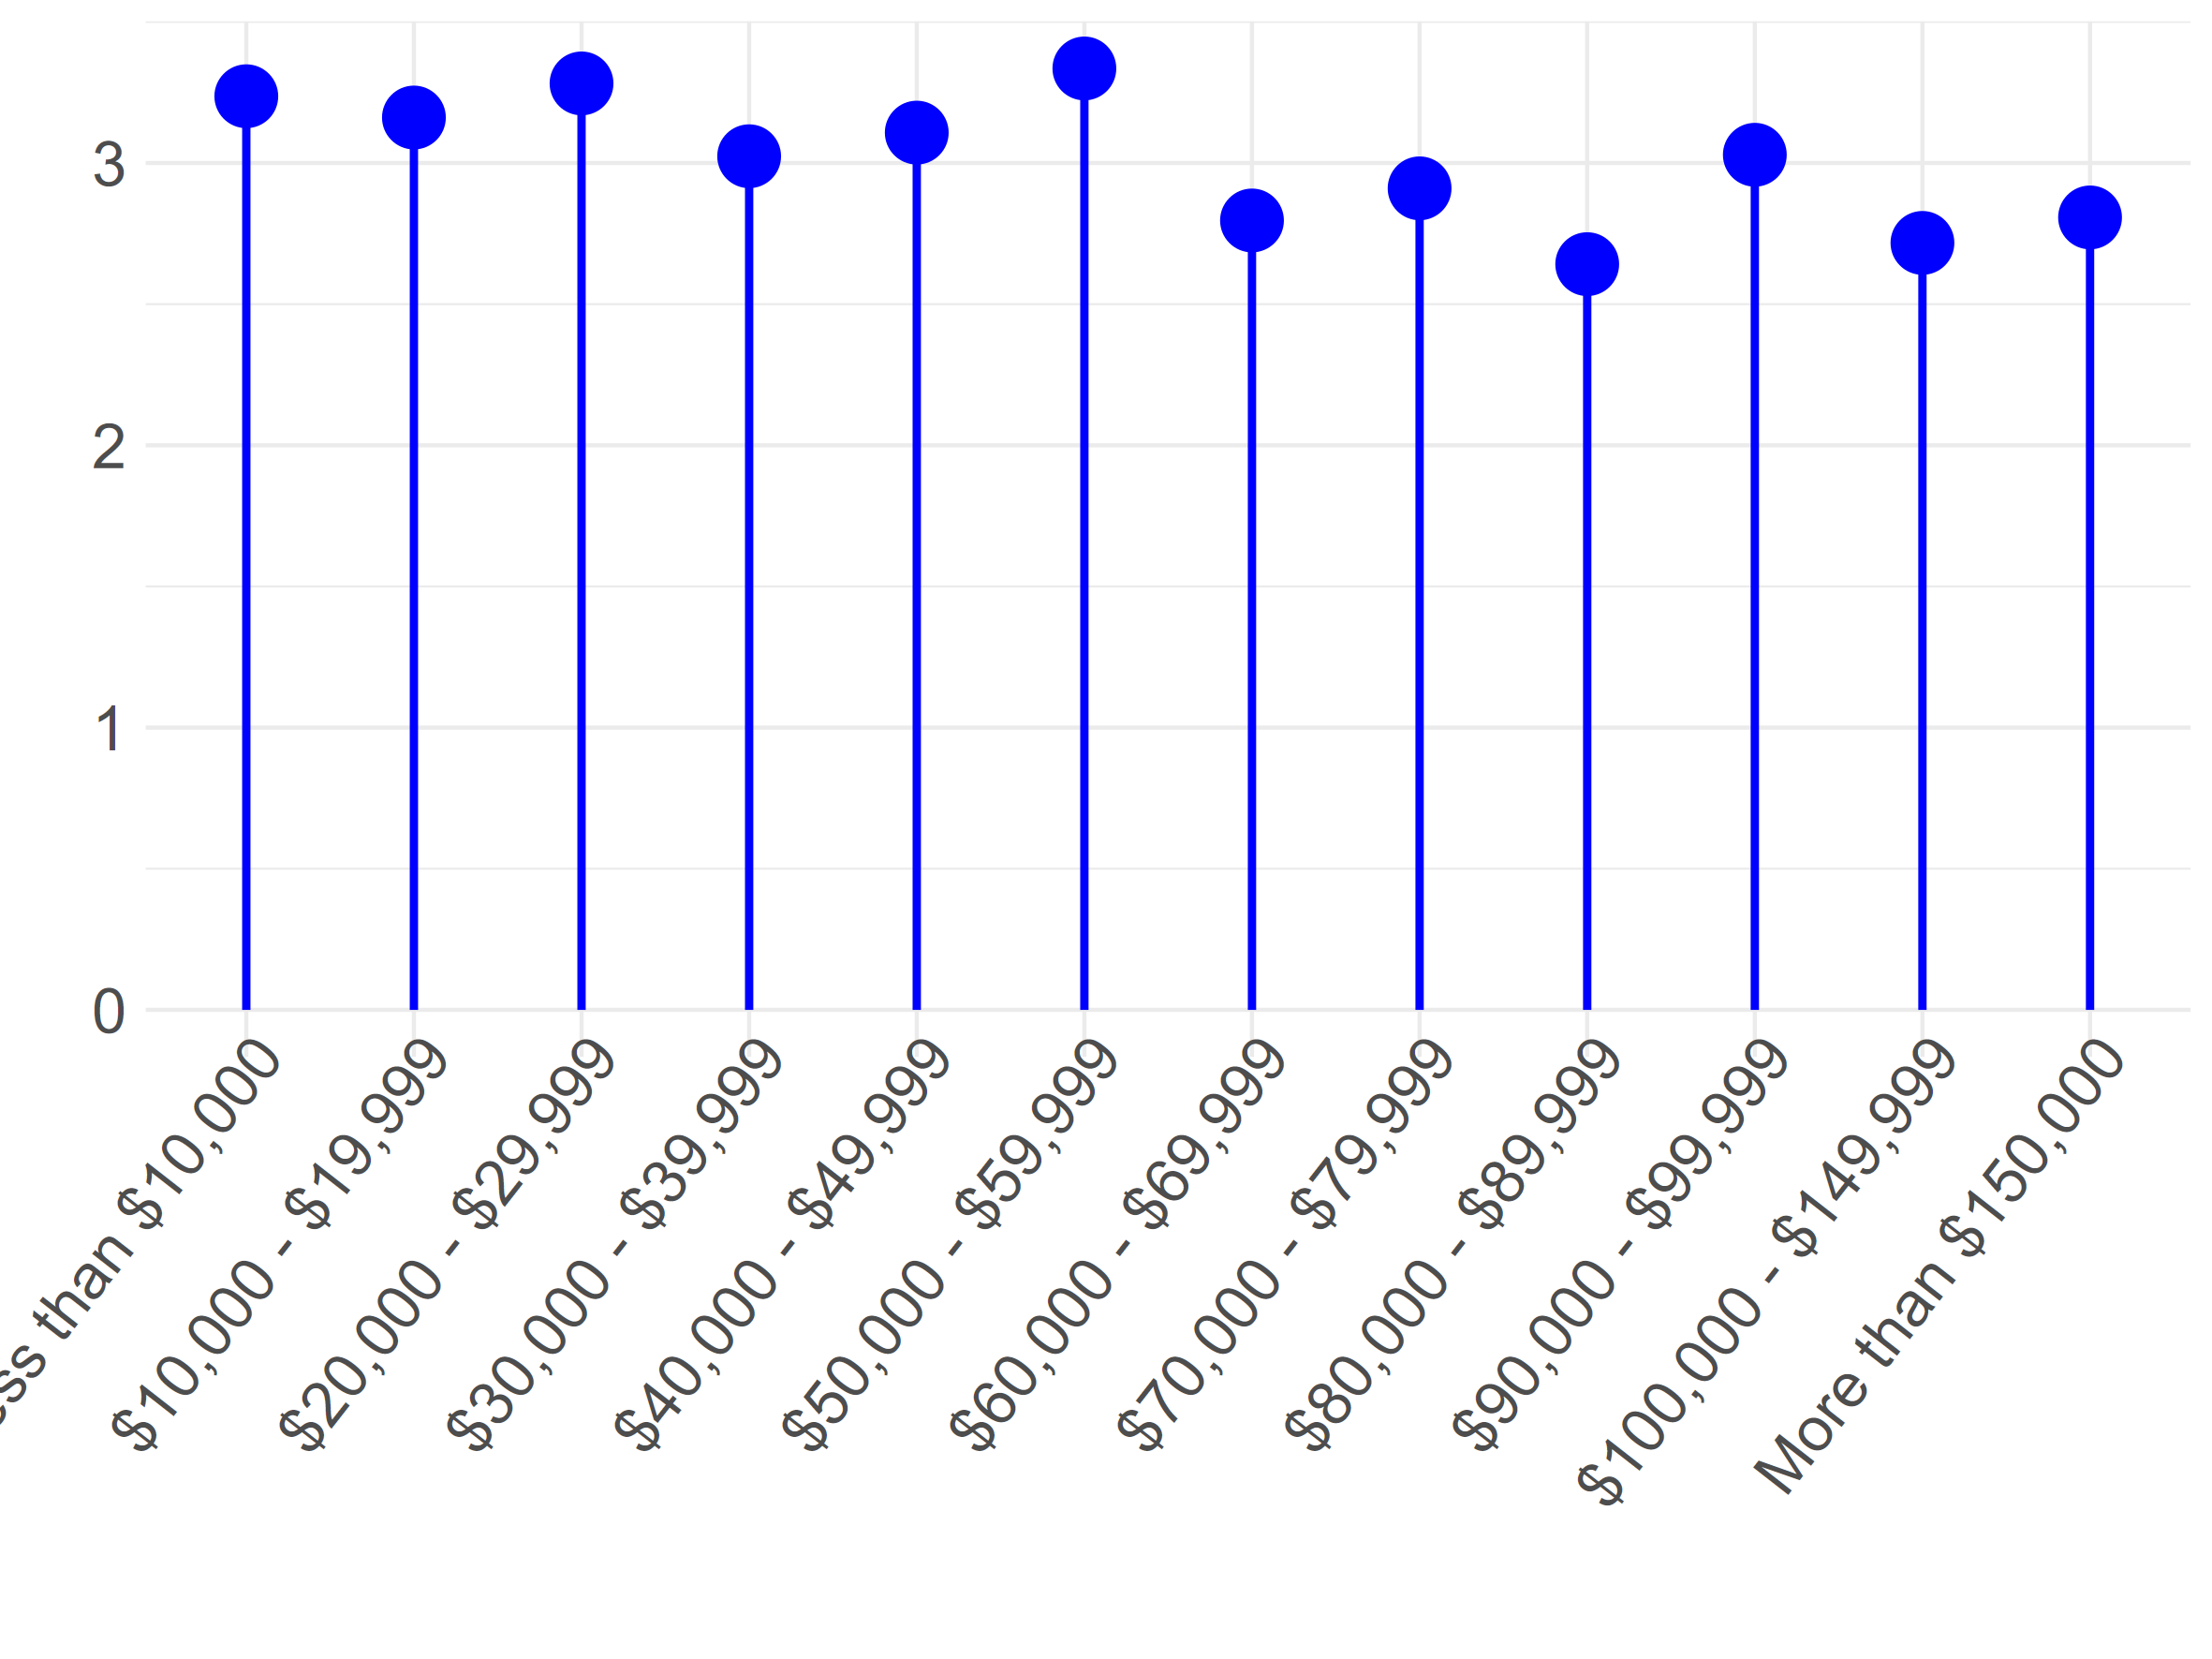
\includegraphics[width=1.0\textwidth]{Plots/uni-dist-grd-int-inc.png}
            \caption{Income}
            \label{fig:grd-int-inc}
    \end{subfigure}
     \begin{subfigure}[b]{0.3\textwidth}
        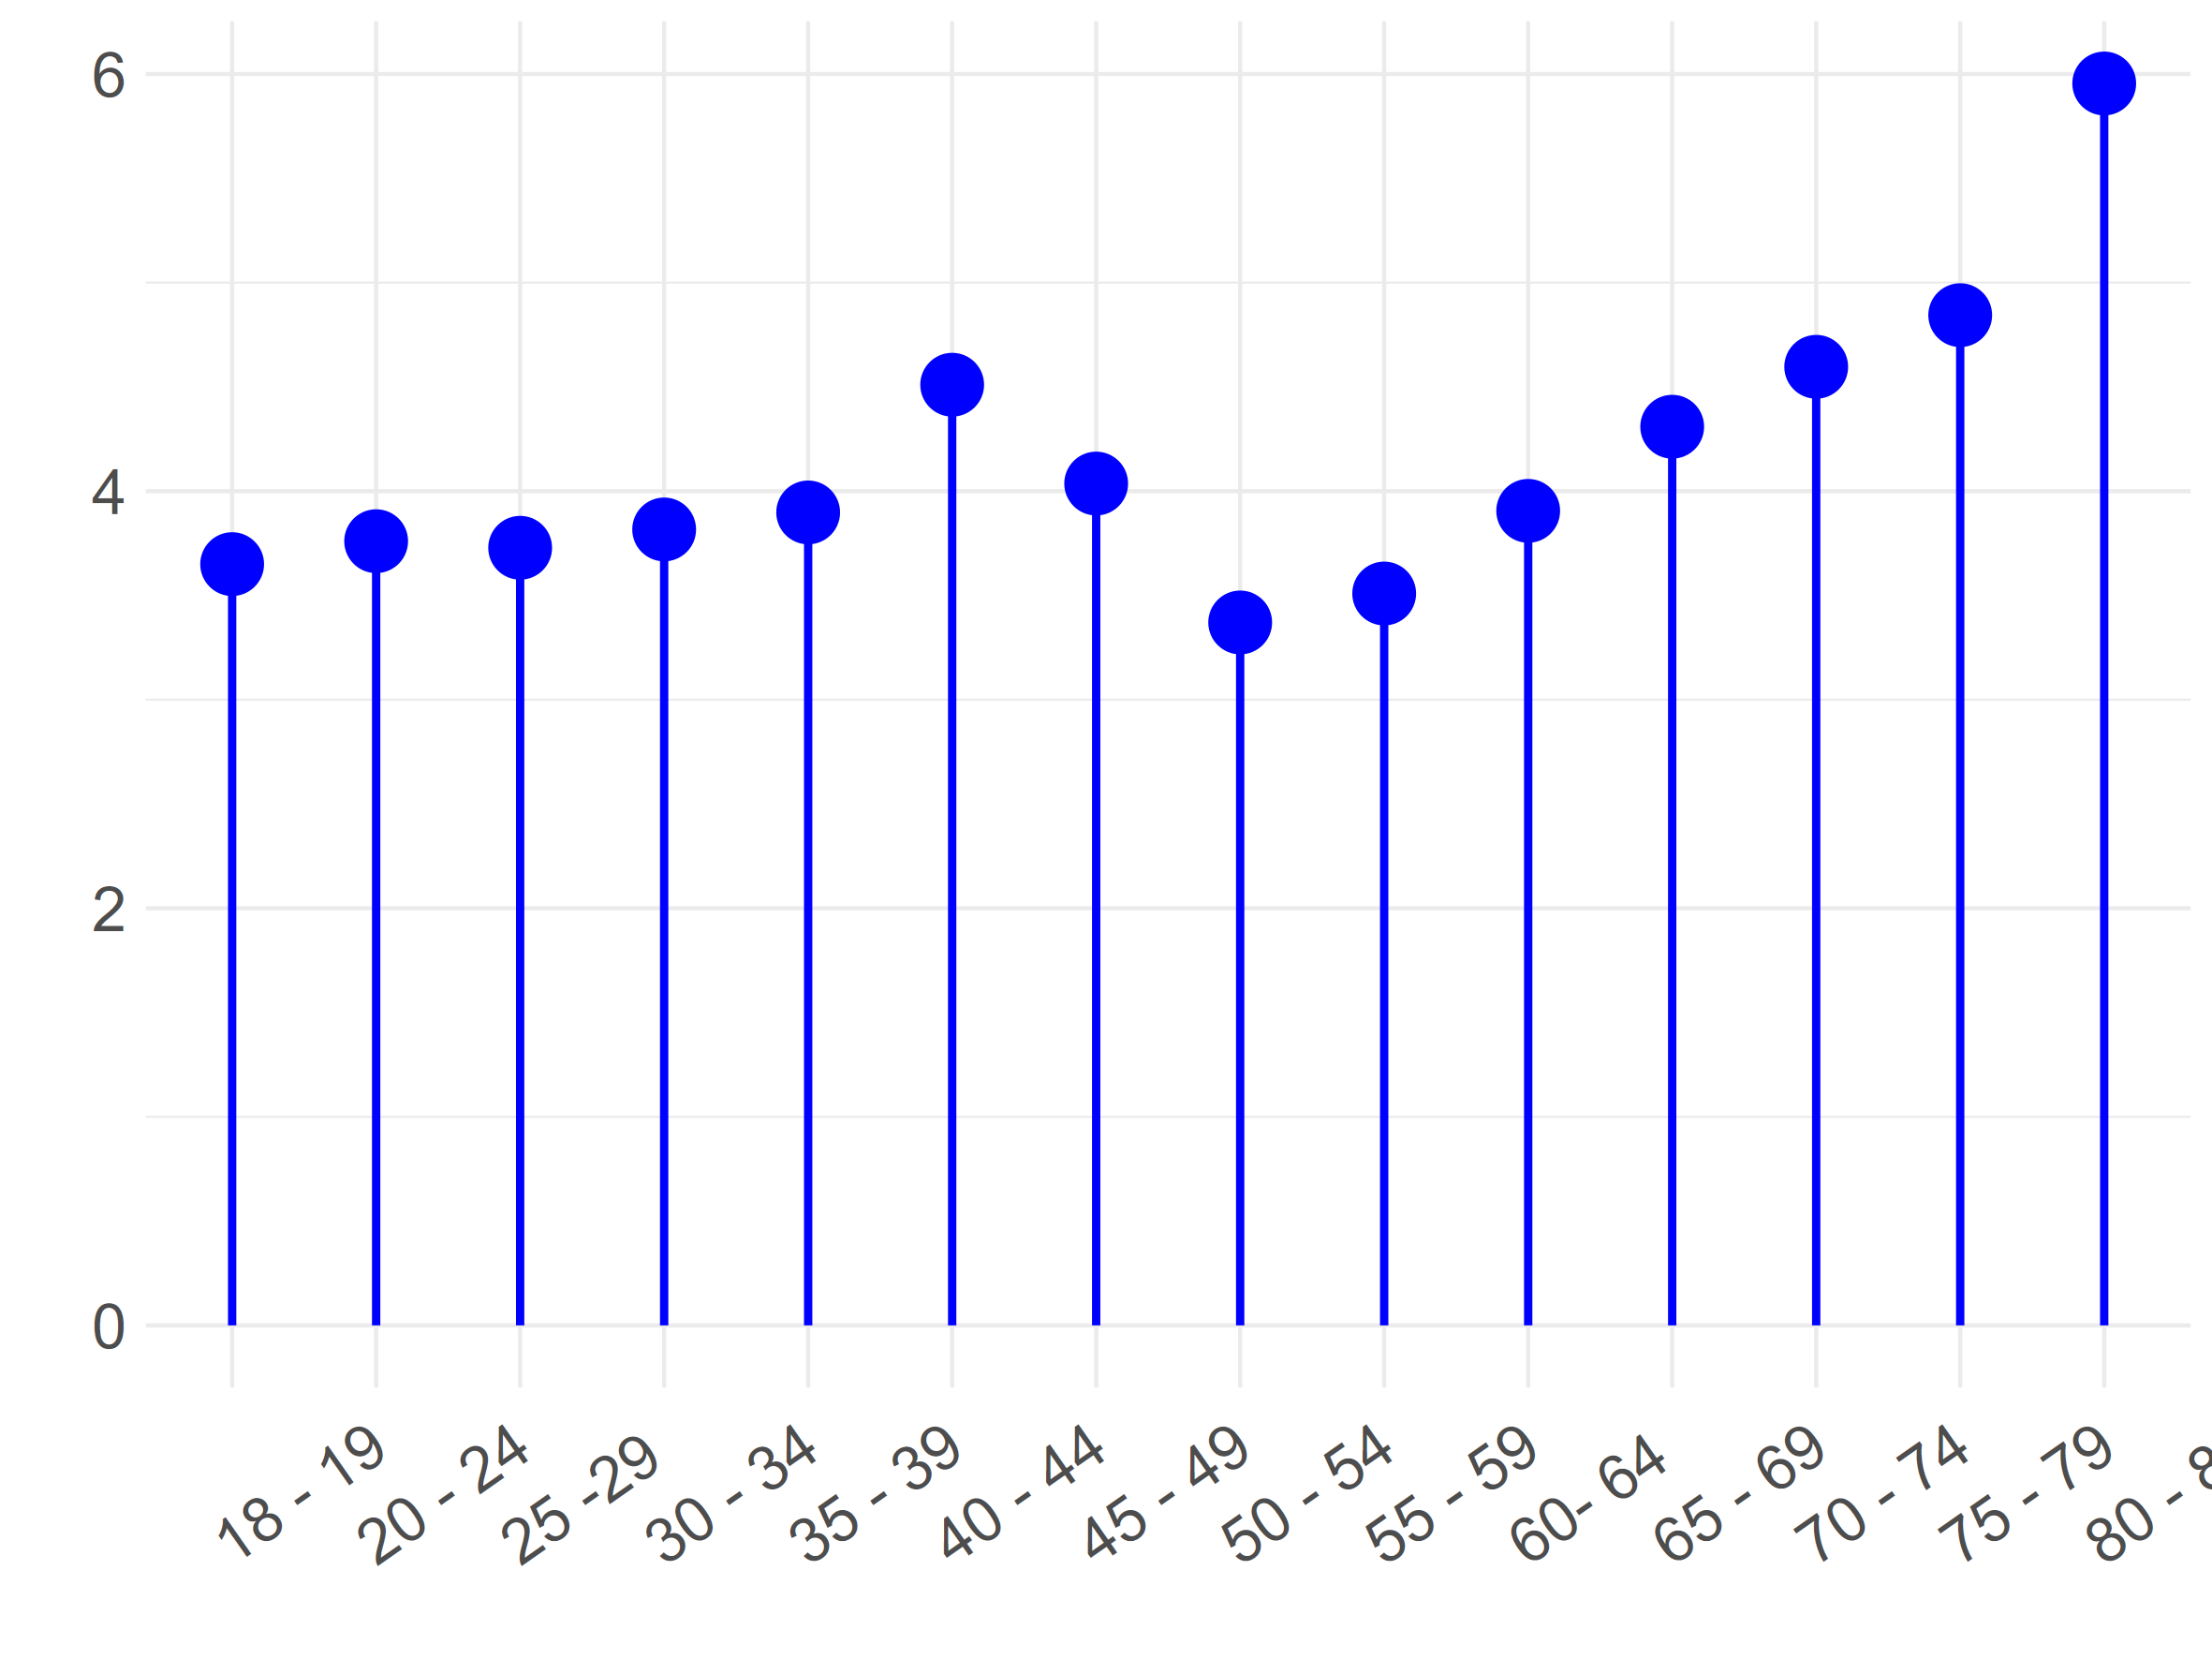
\includegraphics[width=1.0\textwidth]{Plots/uni-dist-grd-int-age.png}
            \caption{Age}
            \label{fig:grd-int-age}
    \end{subfigure}
     \begin{subfigure}[b]{0.3\textwidth}
        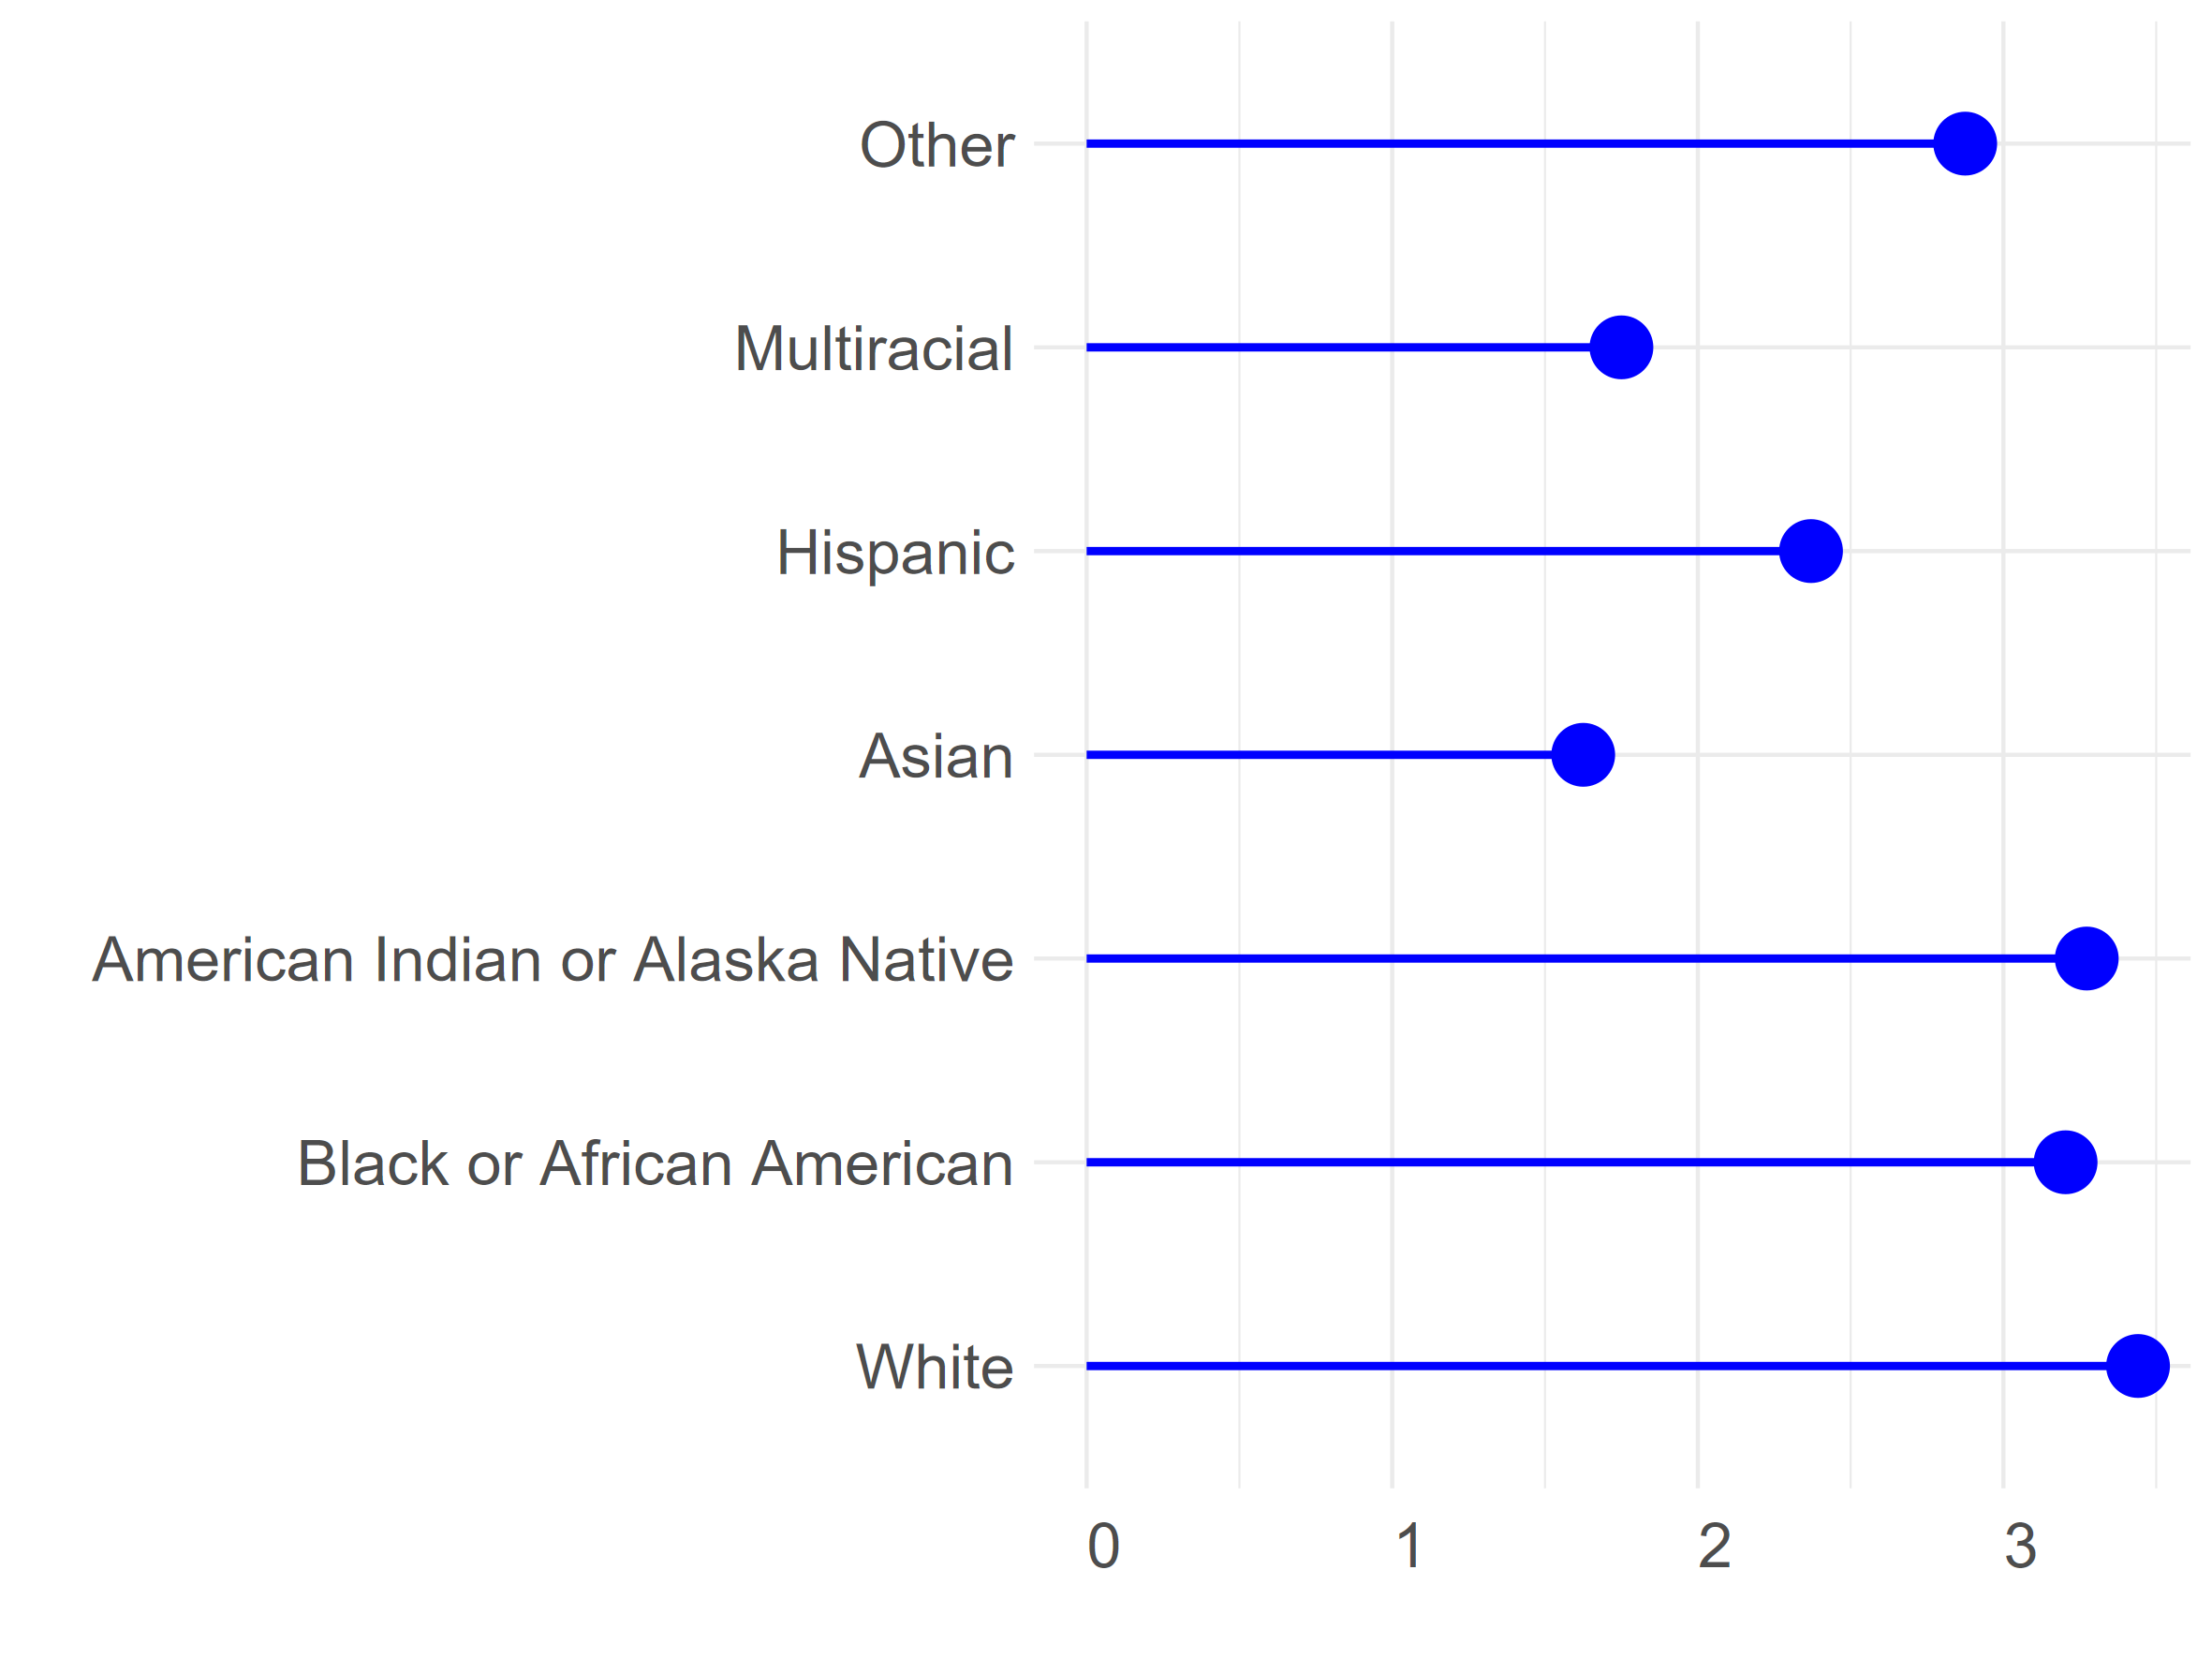
\includegraphics[width=1.0\textwidth]{Plots/uni-dist-grd-int-rac.png}
            \caption{Ethnoracial Identification}
            \label{fig:grd-int-rac}
    \end{subfigure}
     \begin{subfigure}[b]{0.3\textwidth}
        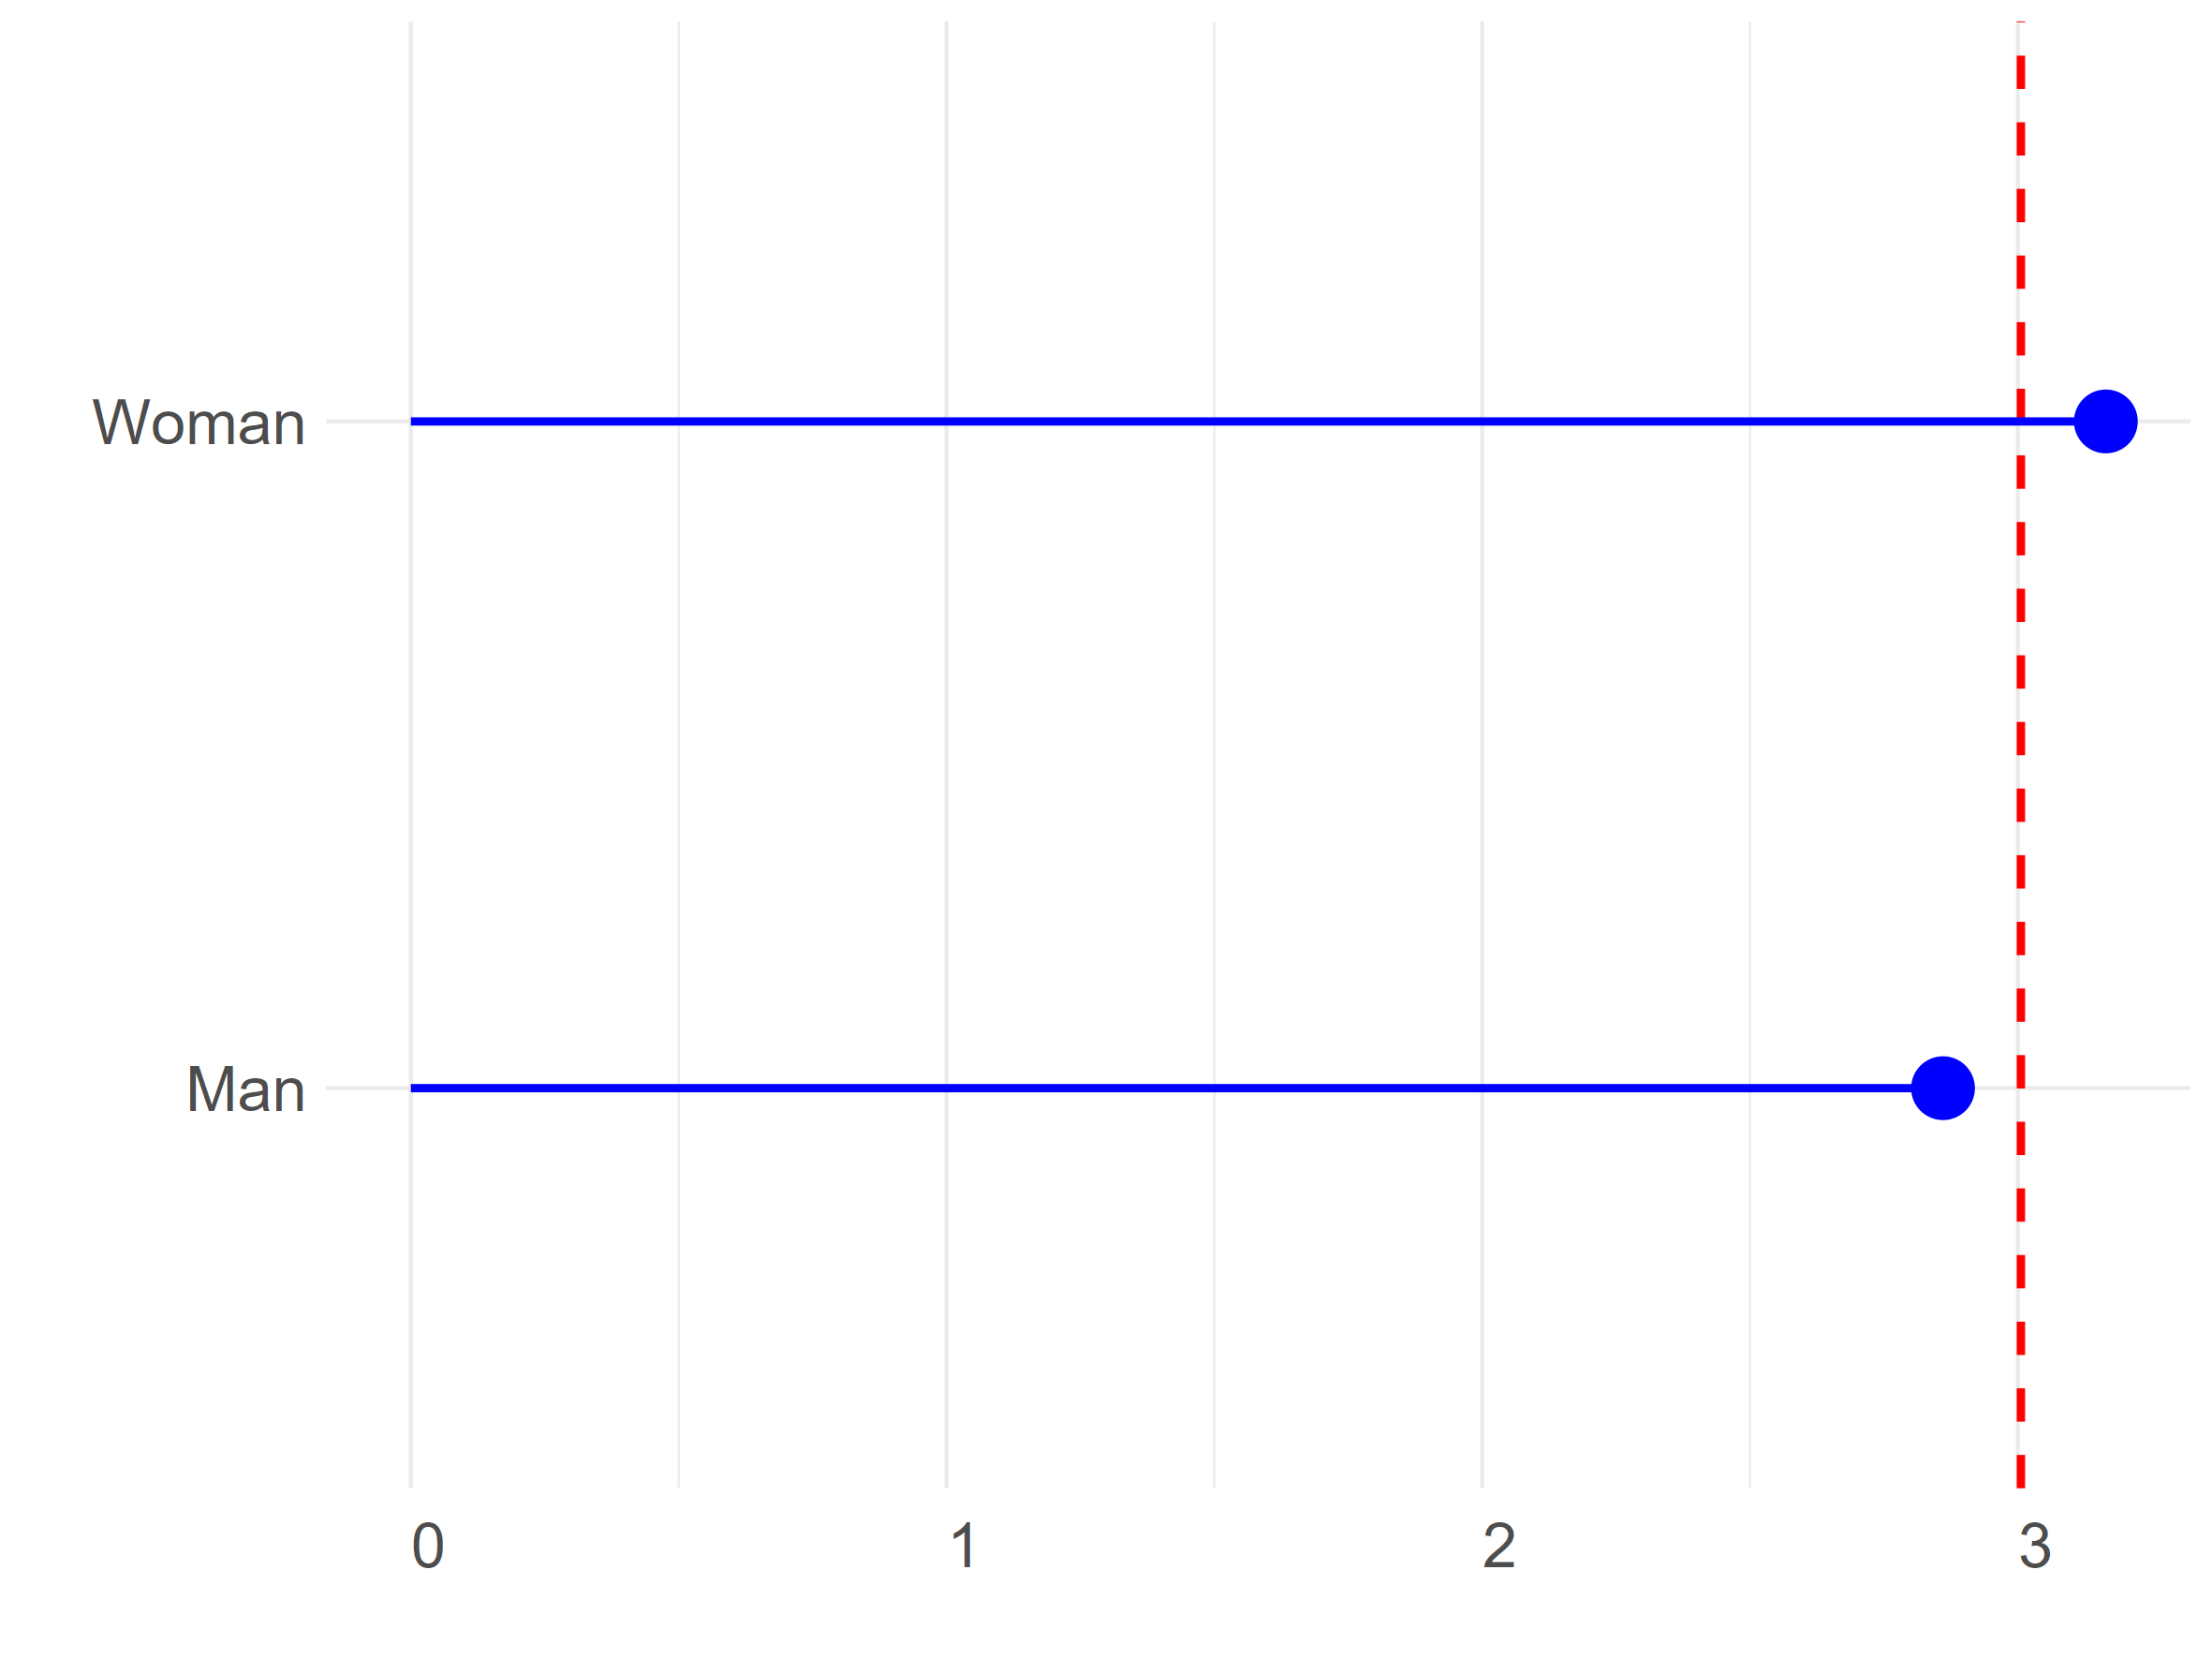
\includegraphics[width=1.0\textwidth]{Plots/uni-dist-grd-int-gen.png}
            \caption{Gender Identification}
            \label{fig:grd-int-gen}
    \end{subfigure}
    \caption{Average number of cultural dislikes across different socio-demographic characteristics.}
    \label{fig:grd-int}
\end{figure}

Symbolic exclusion tendencies among different groups can be straightforwardly attributed to age and education, with older, less educated respondents expressing more dislikes than younger, more educated ones. Importantly, symbolic exclusion is also structured by political ideology in the expected direction---see \citet{rawlings2023polarization-0af}---with liberals being less likely to express cultural dislikes than self-identified conservatives. In the same way, non-whites in the sample are less likely to express cultural dislikes (compared to white respondents), while women express more dislikes (compared to those who identify as men). 

\subsection*{Multivariable Analysis Results}
In their original paper, \citet{lizardo2016end-4fb} proposed modeling categorical tolerance and symbolic exclusion jointly as a hurdle process. The basic idea is that categorical tolerants are a distinct slice of the population who are not at risk of engaging in symbolic exclusion (expressing dislikes). Thus, we can statistically model the joint predictors of both tendencies by assuming that there is a set of predictors that drive the probability of being in the categorical tolerant group (thus not being at risk of expressing dislikes), and net of this, there is a second set of predictors that drive the number of dislikes expressed for those who are at risk of doing so. The zero-inflated Poisson model is thus a natural statistical framework for modeling this dual regime data-generating process \citep{zorn1998analytic-6b1}. Since the univariate distribution of cultural dislikes is comparable across samples (see ~\ref{tab:dis-dist}), I pool the three samples to increase statistical power and report results from the pooled sample analysis, including a binary indicator for each survey sample (using the 2021 Prolific sample as the reference category) in each model. I use listwise deletion of cases with missing values for the socio-demographic covariates included in the model, which leaves us with a total analytical sample of $N = 2091$.

\begin{table}
    \caption{Coefficient Estimates from Zero-Inflated Poisson Models Predicting Categorical Tolerance and Symbolic Exclusion, Joint Prolific and Lucid Samples.}
    \centering
    
\includegraphics[trim={0 0cm 45cm 0},clip, width=0.9\textwidth]{Tabs/zinf-reg.png}
    \label{tab:zinf}
\end{table}

In line with this analytic strategy, Table~\ref{tab:zinf} shows the coefficient estimates from a set of four zero-inflated Poisson regression models. The specifications in each model, for both the count and zero-inflated components, are informed by the descriptive patterns we considered in Figures~\ref{fig:cat-tol} and~\ref{fig:grd-int}. Coefficient estimates corresponding to the count part of the model---predicting the number of dislikes among those who are at risk of expressing them---are shown in the top half of the table. Coefficient estimates for the zero-inflation part of the model, predicting the odds of landing in the categorical tolerant group---and thus not being at risk of engaging in symbolic exclusion---are presented in the lower half of the table. In all models, age, education, income, and political ideology (with higher values indicating a more liberal stance) are entered as ordered numerical inputs. Race (White) and Gender (Female) are entered into the model as dummy indicators. The zero-inflated specifications also contain squared terms for education and income to model expected curvilinear effects (see Figures~\ref{fig:cat-tol-edu} and~\ref{fig:cat-tol-inc}). Finally, I include indicator variables for each of the surveys (one for the 2023 Prolific sample and another for the 2025 Lucid sample), with the Prolific survey conducted in 2021 as the reference category. 

Let us begin with the predictors of symbolic exclusion. Model one includes all of the main socio-demographic predictors. The results align with expectations derived from the descriptive patterns considered earlier. Age increases the likelihood of engaging in symbolic exclusion, but education and income reduce this tendency. Nevertheless, the education effect, as suggested by Figure~\ref{fig:cat-tol-edu}, is substantively small and not statistically significant ($p = 0.09$) using the traditional cutoff value of $p < 0.05$, and becomes smaller and crosses the threshold to decidedly not statistically significant in later specifications. Being politically liberal, on the other hand, has a substantively significant effect, one that is robust---in terms of statistical significance---across models. As suggested by Figure~\ref{fig:cat-tol-pol}, self-identified Liberals are less likely to engage in symbolic exclusion than conservatives. These results indicate that in the United States today, political liberalism is a more reliable predictor of whether a person will engage in symbolic exclusion than is educational attainment, a situation quite different from that which obtained in the 1990s \citep{bryson1996anything-311}. When it comes to ethnoracial identity, self-identified white respondents are more likely to express dislikes compared to respondents who identified with one of the non-white ethnoracial categories ($p < 0.01$). Finally, there is no appreciable gender-identity difference in the propensity to engage in symbolic exclusion via cultural dislikes ($p = 0.52$).

Model 1 includes age as the sole predictor in the zero-inflated part of the model, providing strong evidence that categorical tolerance is primarily a cultural habit among the young and is less prevalent among older respondents ($p < 0.001$). Model 2 includes race and gender as additional predictors of categorical tolerance, verifying the expectation that white respondents are less likely to be found in this group (compared to non-white respondents) and women are less likely to be categorical tolerants (compared to respondents who identify as men). Model 3 introduces education as an additional predictor of categorical tolerance, including a linear input for the respondent's education and a square term for the same covariate. The results verify the idea, suggested by Figure~\ref{fig:cat-tol-edu}, the education effect on the odds of being a categorical tolerant is parabolic, with a negative linear component (indicating that lower education person are more likely to be in the categorical tolerant group) and a positive squared component (indicating that at some point the negative effect reverses, and very high-education individuals end up over-represented among the categorical tolerants). 

That said, the linear component of education is of only marginal statistical significance in Model 3 ($p = 0.07$). This suggests that the bulk of the systematic effect of education is contained in the positive quadratic component, indicating a larger propensity of the very highly educated to be over-represented among categorical tolerants. This impression is confirmed in Model 4, which adjusts for the non-linear effect of self-reported family income on the odds of being a categorical tolerant. Once we do that, the main negative linear effect of education is attenuated ($p = 0.22$), but the exponential positive effect remains ($p < 0.05$), using statistical significance as a criterion. Both components of the income effect, on the other hand, have a statistically significant impact on the odds of being classified as a CT, with a negative linear effect and a positive quadratic effect, suggesting an under-representation of people in middle-income categories among the categorically tolerant. 

\begin{figure}[ht!]
    \captionsetup[subfigure]{font=footnotesize,labelfont=footnotesize}
    \centering
     \begin{subfigure}[b]{0.49\textwidth}
        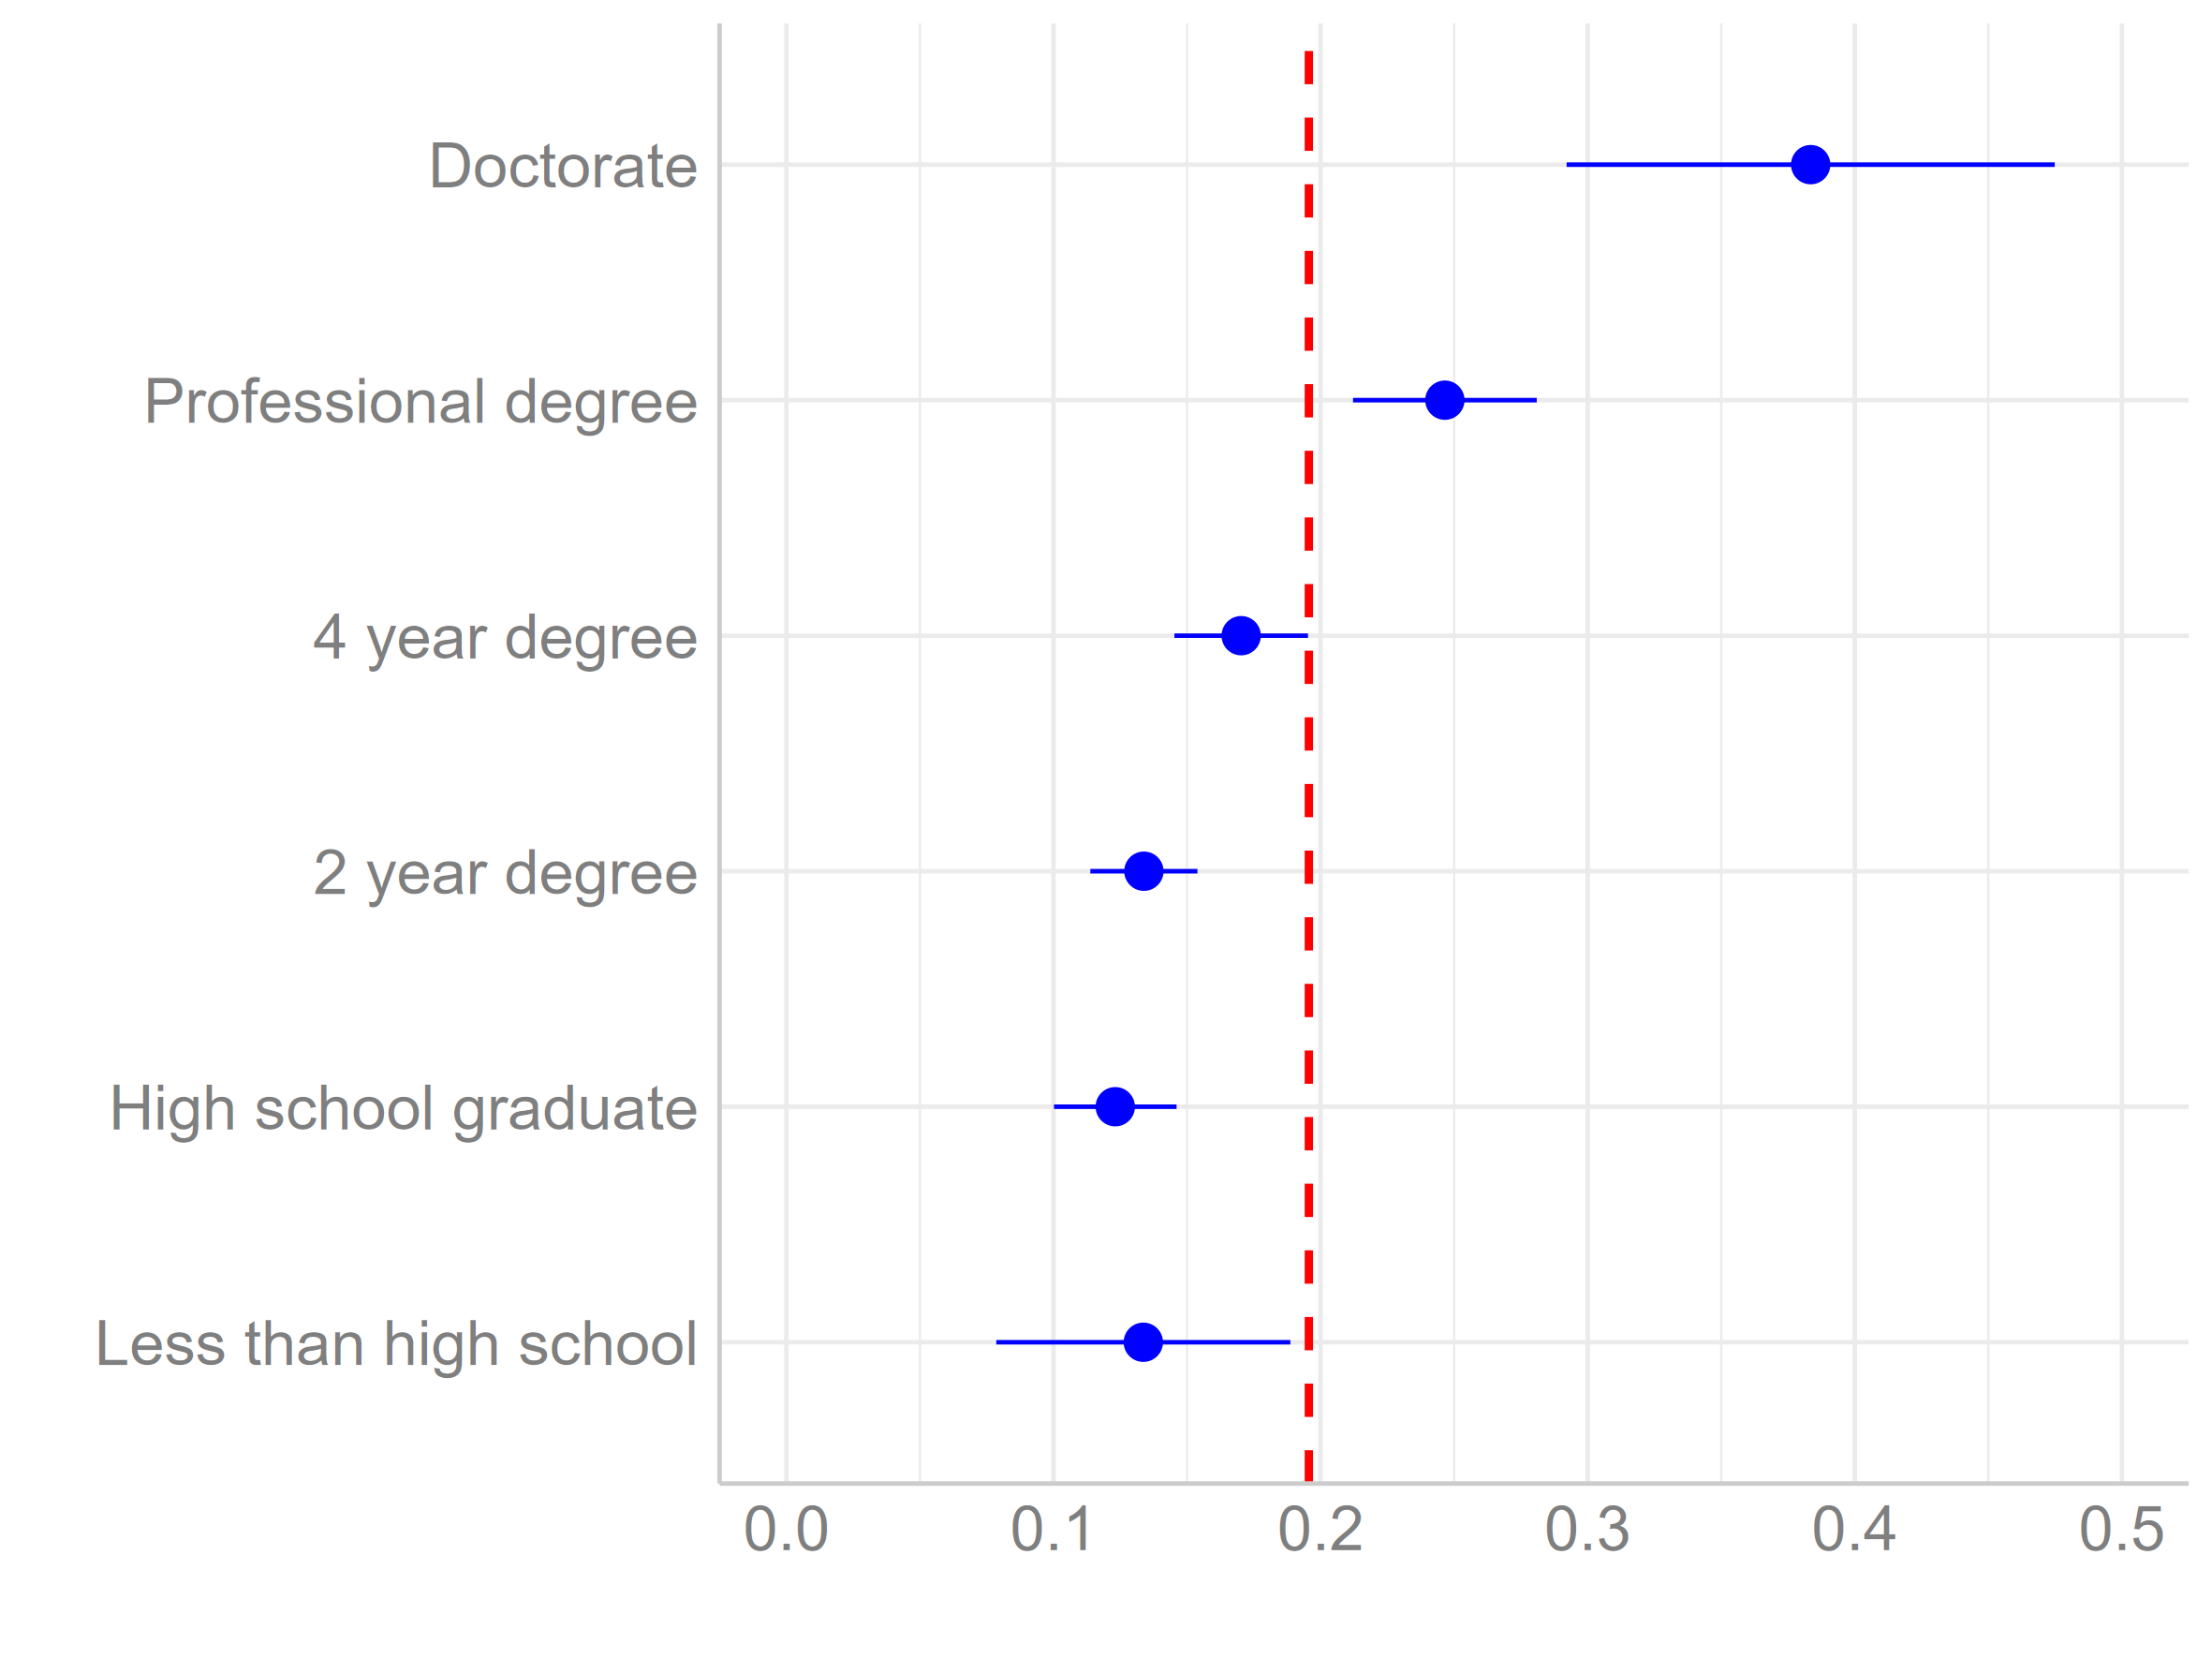
\includegraphics[width=1.0\textwidth]{Plots/educ-pred-plot.png}
            \caption{Highest Degree Completed}
            \label{fig:marg-educ}
    \end{subfigure}
     \begin{subfigure}[b]{0.49\textwidth}
        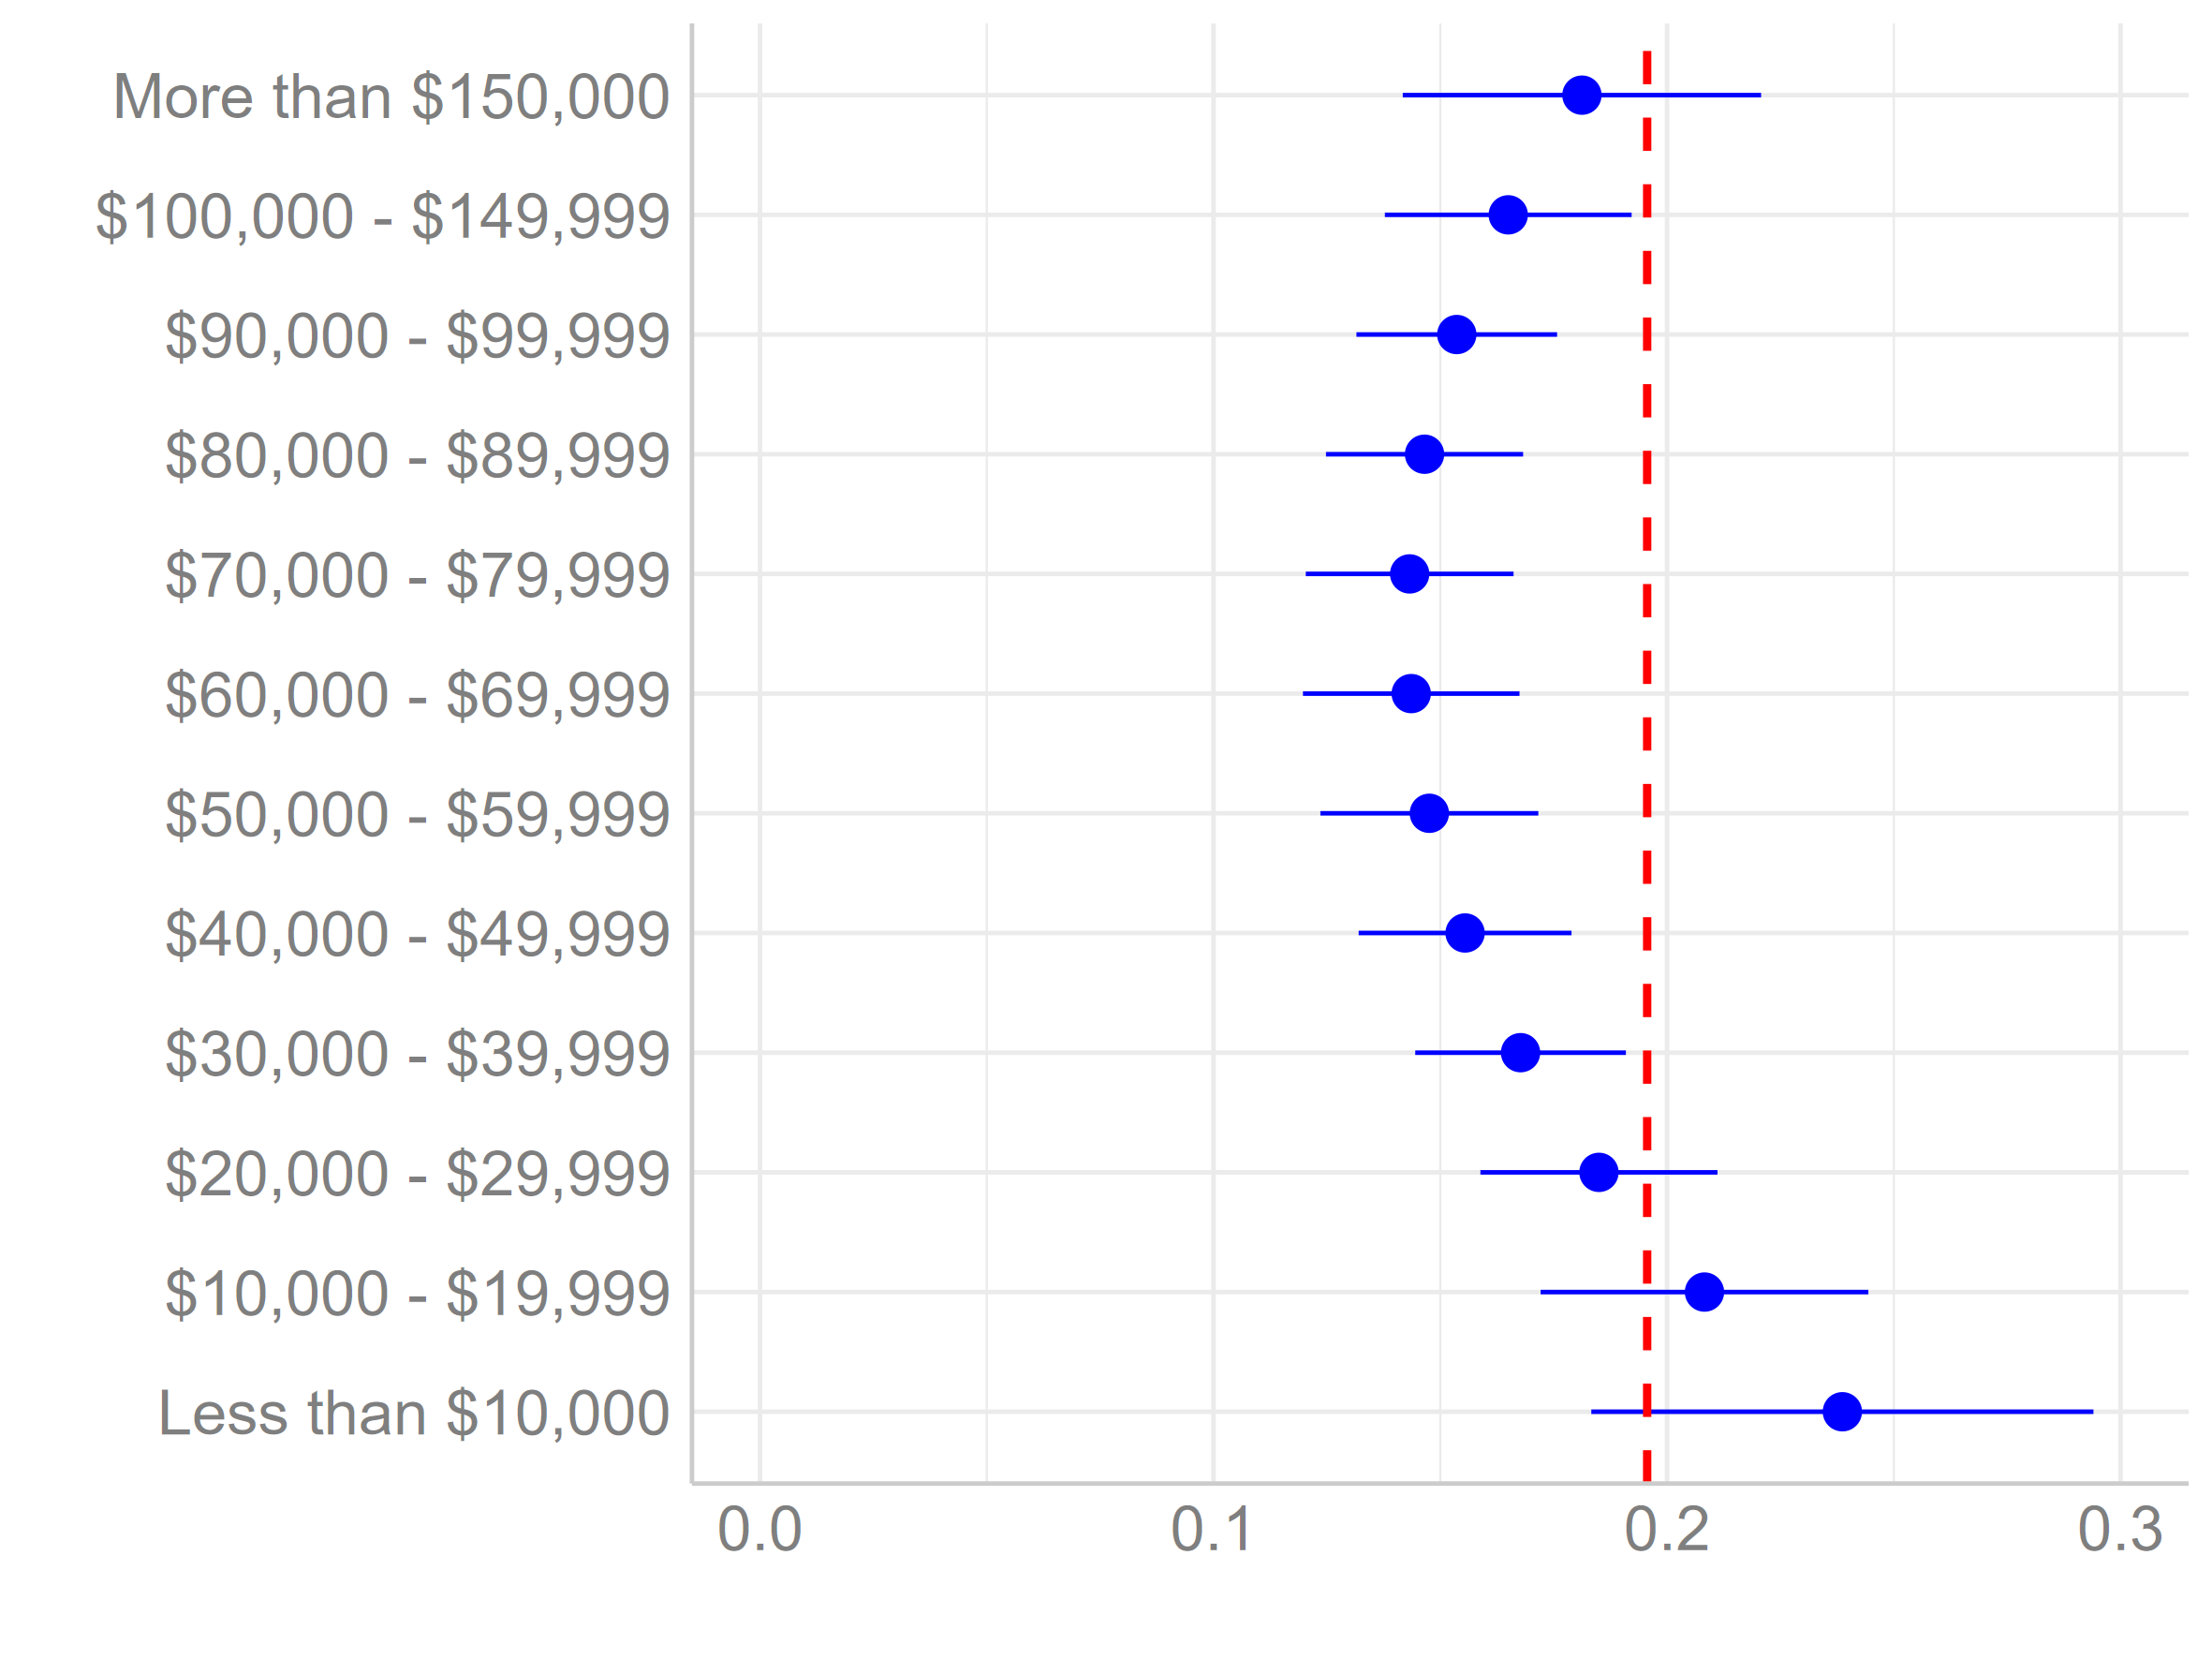
\includegraphics[width=1.0\textwidth]{Plots/inc-pred-plot.png}
            \caption{Family Income}
            \label{fig:marg-inc}
    \end{subfigure}
    \caption{Predicted marginal means of the probability of being a categorical tolerant for education and income groups obtained from the estimates of Model 4 of Table~\ref{tab:zinf}.}
    \label{fig:marg-effects}
\end{figure}

To facilitate the interpretation of the non-linear education and income effects, Figure~\ref{fig:marg-effects} shows marginal effects estimates of the probability of ending up in the categorically tolerant group holding all other predictors at their observed means.\footnote{Estimated using the \texttt{ggeffects} package in \textit{R}.} As we can see, in Figure~\ref{fig:marg-educ}, while the effect of education is non-linear, it is monotonic, suggesting that people with the most advanced levels of education (Professional degree or PhD) are over-represented among the categorical tolerants. This contrasts with the pattern of results obtained by L\&S using data from 2012, suggesting a Bourdieusian upgrading of categorical tolerance as an elite taste pattern in the U.S. today. The income effect, on the other hand, is parabolic along the observed range, suggesting that middle-income people are under-represented among the categorically tolerant, but not indicating any over-representation of very low or very high-income people in this category, who are instead at the observed average proportion for the sample. 

\section*{Discussion and Concluding Remarks}

\subsection*{Summary of Key Results and Limitations}

The findings presented in this paper offer a critical update to the scholarship concerning cultural taste patterns in the United States, particularly the dynamic processes of inclusion and exclusion in musical preferences centered around the idea of Categorical Tolerance (CT) as an emergent taste pattern among Americans. The core empirical results confirm the enduring relevance and continuous expansion of CT, a cultural pattern first identified in earlier work by L\&S \citeyearpar{lizardo2016end-4fb}. The analysis shows that CT continues its ``onward march" among Americans. Specifically, approximately twenty percent of respondents across the samples systematically refused to report disliking any of the measured cultural genres. This prevalence confirms that the univariate distribution of dislikes maintains the expected structure, showing an excess number of zeros and diverging from a simple Poisson process.

The persistence of CT is strongly linked to cohort replacement dynamics, as evidenced by the overrepresentation of younger adults among categorical tolerants relative to older cohorts. Furthermore, consistent with previous analyses, non-white respondents remain overrepresented within the CT group. This tendency suggests that the refusal to engage in symbolic exclusion is sustained as a macro-level pattern of cultural change driven by younger non-white respondents. A particularly salient development in the social patterning of CT is its observed ``trickle-up" of CT into higher educated strata, indicating potentially shifting bases of elite cultural engagement. Unlike L\&S's earlier findings, which noted a slight underrepresentation of college-educated individuals among CTs, the current results show that those reporting the highest levels of education are now overrepresented in this group. This implies that Bourdieusian dynamics of status display, characterized by an embrace of ``conspicuous openness to diversity," may be increasingly at play, positioning CT as a valued cultural tool for contemporary elites \citep{jarness2017im-001, ollivier2008modes-96f}.

Beyond status and demographic correlates, the study offers insight into the growing linkage between cultural taste and political orientation \citep{rawlings2023polarization-0af}. While categorical tolerance itself does not appear to be polarized along liberal/conservative lines, the propensity for symbolic exclusion---the act of expressing dislikes---is evidently polarized. Adjusting for other sociodemographic factors, conservatives demonstrate a greater likelihood of expressing more cultural dislikes compared to liberals. This suggests that political ideology, alongside age, has become a reliable predictor of expressing dislikes for cultural genres in the contemporary United States, echoing recent work that identifies increasing polarization involving cultural taste patterns.

One limitation of the present study is the need to compare findings over time using survey instruments with varying scopes. The present study's cultural taste measures rely on a smaller number of genres (twelve) compared to L\&S's original research (eighteen genres in the 2012 survey). This reduction in the item battery introduces caution when making direct comparisons of dislike volumes. Nevertheless, the statistical modeling approach employed here, based on Poisson hurdle models, provides confidence in distinguishing between two distinct populations: categorical tolerants and those at risk of symbolic exclusion.

Furthermore, the theoretical interpretation of CT's meaning remains an area of ongoing sociological investigation and debate, complicated by inherent data constraints. Some comparative research suggests that the refusal to dislike may sometimes indicate non-committal behaviors such as indecisiveness or generalized ambivalence (often captured as ``mixed feelings" or ``do not agree nor disagree"), rather than authentic cosmopolitan tolerance or a genuine embrace of cultural diversity. Indeed, the absence of dislikes may signal a socially unstructured ambivalence that increased over time in other contexts. While the zero-inflated Poisson model was employed to statistically separate the population at risk of exclusion from the categorical tolerants, aiming for a coherent social niche, the underlying disposition---whether strategic status signaling or genuine universal acceptance--cannot be definitively determined by the quantitative measures used.

Additionally, while using broad genre categories is standard in large-scale research in the sociology of taste, this approach necessarily obscures nuances critical to contemporary distinction. Critics point out that focusing solely on genre acceptance risks overlooking within-genre hierarchies, where specific tastes for objects (artists, tracks, specific works) within accepted broad genres are increasingly crucial for symbolic exclusion and status signaling among higher-status groups \citep{childress2019encultured-e58, nault2021social-1bf}. Using broad genre categories may therefore limit the ability to fully capture the subtle, exclusive tastes that coexist with inclusive genre preferences in the contemporary configuration of elite cultural consumption \citep{lizardo2024from-ddd}.

\subsection*{Suggestions for Future Work}
The current research suggests several promising directions for future research aimed at deepening our theoretical and empirical understanding of taste, tolerance, and inequality in the contemporary moment. First, moving forward necessitates adopting more fine-grained measurement strategies to overcome the limitations of broad genres. Future research should replicate this work using more specific categorizations, focusing on objects (artists, albums, specific works) rather than just genres, to comprehensively investigate the hypothesized contemporary configuration of high-status tastes. Is categorical tolerance only observed among broad genre categories, or can it also be observed at the level of objects within genres? Such refined analyses are increasingly relevant for understanding how cultural boundaries persist or are redrawn in cultural fields.

Second, more targeted investigations, perhaps using qualitative strategies, are required to definitively unpack the sociological meaning of Categorical Tolerance. Future studies should move beyond measuring the mere volume of likes and dislikes toward qualitative or mixed-methods approaches that capture the underlying motivations or the specific ``mode'' of appropriation of CTs relative to particular objects and practices. This would distinguish between CT as a performance of socially valued openness (e.g., a strategic status performance), a broader cosmopolitan disposition, or simply ambivalence/indecisiveness in taking a stance.

Third, given the robust connection between symbolic exclusion and political ideology, further scholarly attention must be dedicated to tracking this accelerated linkage. Research should continue to monitor how cultural taste patterns are drawn into the ``oil spill" of political polarization \citep{dellaposta2020pluralistic-ed4}. This could involve investigating the processes and mechanisms via which political actors may strategically impose cultural boundaries, thereby reinforcing political cleavages via cultural affinity or distancing.

Finally, future sociological inquiry should broaden its scope to include comparative and contextual replication. While the US context provides specific insights into racial dynamics and high polarization, examining how CT manifests in other nations---such as the recent comparative framework in Finland or social settings outside the Euro-American West like South Korea---could illuminate how local social topography and ethnic divisions modulate the social correlates and meaning of categorical tolerance. Furthermore, exploring whether personality traits, such as those related to openness or extroversion \citep{andrews2022culture-390}, mediate the relationship between cultural exposure and the resulting omnivorous or categorically tolerant dispositions could offer a promising line of interdisciplinary inquiry.

\newpage
\bibliography{references}
\bibliographystyle{asr}

\end{document}
